%%%%%%%%%%%%%%%%%%%%%%%%%%%%%%%%%%%%%%%%%%%%%%%%%%%%%%%%%%%%%%%%%%%
%DIF LATEXDIFF DIFFERENCE FILE
%DIF DEL ./old/main.tex   Tue Dec  4 15:43:26 2018
%DIF ADD main.tex         Mon Feb 11 18:00:52 2019
% Cocca, Giordano,  Vassio
% OCtober 2018
%%%%%%%%%%%%%%%%%%%%%%%%%%%%%%%%%%%%%%%%%%%%%%%%%%%%%%%%%%%%%%%%%%%


\documentclass[review, letterpaper,3p, 11pt]{elsarticle}

\usepackage{amsmath,amssymb,amsfonts}
\usepackage{algorithmic}
\usepackage{graphicx}
\usepackage{textcomp}
\usepackage{hyperref}
\usepackage{xcolor}
\usepackage{url}
\usepackage[ruled]{algorithm2e}
\usepackage{subfigure}
\usepackage{xspace}
\usepackage{setspace}
%DIF 20a20-22
\usepackage{eurosym} %DIF > 
\DeclareMathOperator*{\argmax}{arg\,max} %DIF > 
\DeclareMathOperator*{\argmin}{arg\,min} %DIF > 
%DIF -------

%DIF 21-22d24
%DIF < 
%DIF < 
%DIF -------
\newcommand{\tool}{\textit{UMAP}\xspace}
\newcommand{\github}{\url{https://github.com/michelelt/sim3.0}}
\newcommand{\trace}{\url{www.todo.com}}

% To comment in the paper
\usepackage{color}
\newcommand{\lv}[1]{{\color{cyan}{[luca: #1]}}}
\newcommand{\mc}[1]{{\color{green}{[mike: #1]}}}
\newcommand{\mm}[1]{{\color{red}{[mellia: #1]}}}
\newcommand{\dg}[1]{{\color{orange}{[danilo: #1]}}}
\newcommand{\ext}[1]{{\color{blue}{#1}}}
%DIF 34c35
%DIF < 
%DIF -------
\newcommand{\reviewed}[1]{{\color{blue}{#1}}} %DIF > 
%DIF -------


%% Document starts
%DIF PREAMBLE EXTENSION ADDED BY LATEXDIFF
%DIF UNDERLINE PREAMBLE %DIF PREAMBLE
\RequirePackage[normalem]{ulem} %DIF PREAMBLE
\RequirePackage{color}\definecolor{RED}{rgb}{1,0,0}\definecolor{BLUE}{rgb}{0,0,1} %DIF PREAMBLE
\providecommand{\DIFaddtex}[1]{{\protect\color{blue}\uwave{#1}}} %DIF PREAMBLE
\providecommand{\DIFdeltex}[1]{{\protect\color{red}\sout{#1}}}                      %DIF PREAMBLE
%DIF SAFE PREAMBLE %DIF PREAMBLE
\providecommand{\DIFaddbegin}{} %DIF PREAMBLE
\providecommand{\DIFaddend}{} %DIF PREAMBLE
\providecommand{\DIFdelbegin}{} %DIF PREAMBLE
\providecommand{\DIFdelend}{} %DIF PREAMBLE
%DIF FLOATSAFE PREAMBLE %DIF PREAMBLE
\providecommand{\DIFaddFL}[1]{\DIFadd{#1}} %DIF PREAMBLE
\providecommand{\DIFdelFL}[1]{\DIFdel{#1}} %DIF PREAMBLE
\providecommand{\DIFaddbeginFL}{} %DIF PREAMBLE
\providecommand{\DIFaddendFL}{} %DIF PREAMBLE
\providecommand{\DIFdelbeginFL}{} %DIF PREAMBLE
\providecommand{\DIFdelendFL}{} %DIF PREAMBLE
%DIF END PREAMBLE EXTENSION ADDED BY LATEXDIFF
%DIF PREAMBLE EXTENSION ADDED BY LATEXDIFF
%DIF HYPERREF PREAMBLE %DIF PREAMBLE
\providecommand{\DIFadd}[1]{\texorpdfstring{\DIFaddtex{#1}}{#1}} %DIF PREAMBLE
%\providecommand{\DIFdel}[1]{\texorpdfstring{\DIFdeltex{#1}}{}} %DIF PREAMBLE
%DIF END PREAMBLE EXTENSION ADDED BY LATEXDIFF
\providecommand{\DIFdel}[1]{} % Don't show deleted text

\begin{document}
\doublespacing

\begin{frontmatter}


\title{Free Floating Electric Car Sharing Design: \\Data Driven Optimisation}
\tnotetext[t1]{This document is an extension of our previous work \cite{taormina} presented at IEEE SMARTCOMP 2018.}
%\tnotetext[t2]{Authors are listed in alphabetical order.}


\author[poli]{Michele Cocca}
\ead{michele.cocca@polito.it}
\author[dauin]{Danilo Giordano}
\ead{danilo.giordano@polito.it}
\author[poli]{Marco Mellia}
\ead{marco.mellia@polito.it}
\author[poli]{Luca Vassio}
\ead{luca.vassio@polito.it}


\address[poli]{Department of Electronics and Telecommunications, Politecnico di Torino, Italy.}
\address[dauin]{Department of Control and Computer Engineering, Politecnico di Torino, Italy.}


\begin{abstract}
\DIFdelbegin %DIFDELCMD < 

%DIFDELCMD < %%%
\DIFdelend %Self-contained abstract of no more than 100 words MA HO VISTO CHE NEGLI ALTRI PAPER NE USANO CIRCA 180, outlining the aims, scope and conclusion of the paper. Three to five keywords must be included.
\DIFdelbegin %DIFDELCMD < 

%DIFDELCMD < %%%
%DIF < Free Floating Car Sharing (FFCS) is a transport paradigm where  customers are free to rent and drop cars of a fleet within city limits. 
\DIFdelend %DIF > Ora siamo a 209

In this work we consider the design of a Free Floating Car Sharing (FFCS) system based on Electric Vehicles. We face the problems of finding the optimal placement of charging stations, and the design of smart car return policies, i.e, how many and where to place charging stations, and whether to ask or not customers to \DIFdelbegin \DIFdel{connect }\DIFdelend \DIFaddbegin \DIFadd{return }\DIFaddend the car to a charging pole.

\DIFdelbegin \DIFdel{For this, we leverage data of }\DIFdelend \DIFaddbegin \DIFadd{We leverage actual data containing rentals performed by }\DIFaddend Car2Go \DIFdelbegin \DIFdel{, a worldwide FFCS provider}\DIFdelend \DIFaddbegin \DIFadd{customers}\DIFaddend . We obtain information for \DIFdelbegin \DIFdel{two }\DIFdelend \DIFaddbegin \DIFadd{several }\DIFaddend months worth of actual \DIFdelbegin \DIFdel{rentals from customers }\DIFdelend \DIFaddbegin \DIFadd{trips }\DIFaddend in the city of Turin, our use case.
Via \DIFdelbegin \DIFdel{accurate }\DIFdelend trace driven simulations, we replay the exact same trips while simulating electric car based FFCS, to accurately gauge battery discharging and recharging.
With this, we compare different charging station \DIFdelbegin \DIFdel{placement algorithms, guided by domain knowledge, or driven by global }\DIFdelend \DIFaddbegin \DIFadd{placements, also driven by }\DIFaddend optimisation algorithms. \DIFdelbegin \DIFdel{We also }\DIFdelend \DIFaddbegin \DIFadd{Moreover, we }\DIFaddend observe the impact of collaborative or selfish car return policies.

Results are surprisingly: just \DIFaddbegin \DIFadd{as few as 13 charging stations (52 poles) guarantee a fleet of  377 }\DIFaddend vehicles running in a 1 million inhabitant city to work flawlessly, with limited customer's discomfort.
We believe our data driven methodology helps researchers and car sharing providers discerning different design solutions. For this, we make available all data and tools to foster further studies in these directions.


\end{abstract}

\begin{keyword}
car sharing \sep electric vehicle \sep data driven optimisation\sep charging station placement\sep free floating
\end{keyword}

\end{frontmatter}

\section{Introduction}
\label{sec:intro}

%1) IMPORTANZA DI PASSARE A MOBILITA CONDIVISA E A VEICOLI ELETTRICI
%\lv{1) IMPORTANZA DI PASSARE A MOBILITA CONDIVISA E A VEICOLI ELETTRICI}

Mobility and pollution are challenging problems in our cities. Private vehicles, still  \DIFdelbegin \DIFdel{an }\DIFdelend important urban transportation means, are among the major contributors to both congestion and air pollution. Because of this, smart and shared mobility are seen as a key component to reduce emissions and traffic~\cite{Firnkorn2011}.
Given a fleet of cars, Free Floating Car Sharing (FFCS) systems allow customers to pick and drop a shared car everywhere inside an operative area, thus reducing the number of private cars and increasing the number of available parking spots.
The conversion from internal combustion cars into Electric Vehicles \DIFaddbegin \DIFadd{(EVs) }\DIFaddend is seen as the next big opportunity to drastically reduce pollution inside urban areas~\cite{FM15}. However, the design of a system based on electric cars entails the deployment of a charging station network\DIFdelbegin \DIFdel{, whose design is challenging given the lengthy battery recharging operation}\DIFdelend ~\cite{plugPowers}.

%%%%2) PROBLEMI DI FFCS E OBIETTIVI GENERALI
%\lv{2) PROBLEMI DI FFCS E OBIETTIVI GENERALI}

In this work, we tackle the design of an electric FFCS system.
This is a challenging problem, given charging constraints which impact car availability, and the cost of the infrastructure setup and maintenance.
The design of the charging station infrastructure requires thus ingenuity to maximise customers' comfort, and minimise cost for the operator~\cite{PlacementAndPowergrid,placementAustin,mipCSPpechino}. 

Two are the main problems that need to be faced: i) the charging station placement problem, i.e., how many and where to install charging stations; and ii) the return policy customers have to follow at the end of the rental, i.e., in which cases to ask the customer to return the car to a charging station.
In this paper we face both the above problems. \DIFaddbegin \DIFadd{Notice that the number of charging stations is directly related to system installation costs.
}\DIFaddend 

We strongly believe actual usage data is fundamental to answer these questions. While in the past some works have proposed solutions for the design of electric FFCS~\cite{FM15,WB15}, we are among the first to take a complete data-driven approach~\DIFdelbegin \DIFdel{\mbox{%DIFAUXCMD
\cite{PlacementAndPowergrid,placementAustin,mipCSPpechino,ChargingStationForVehicularNetworks}}%DIFAUXCMD
}\DIFdelend \DIFaddbegin \DIFadd{\mbox{%DIFAUXCMD
\cite{PlacementAndPowergrid,placementAustin,mipCSPpechino,ChargingStationForVehicularNetworks,3_RickenbergGebhardtBreitner_2013,5_SonnebergKune_2015} }%DIFAUXCMD
in an electric FFCS}\DIFaddend . Here, we extend our preliminary \DIFdelbegin \DIFdel{work~\mbox{%DIFAUXCMD
\cite{taormina} }%DIFAUXCMD
}\DIFdelend \DIFaddbegin \DIFadd{works~\mbox{%DIFAUXCMD
\cite{taormina, maui} }%DIFAUXCMD
}\DIFaddend by presenting a more extensive evaluation, and introducing two \DIFdelbegin \DIFdel{global }\DIFdelend search algorithms.

We start by describing the system we implemented to collect real data from the \DIFdelbegin \DIFdel{actual }\DIFdelend FFCS systems currently in use in the city of Turin  (Italy), which we consider as a test case. Despite being based on \DIFdelbegin \DIFdel{traditional combustion engines}\DIFdelend \DIFaddbegin \DIFadd{internal combustion engine cars}\DIFaddend , this data perfectly captures the actual usage patterns of regular customers~\cite{UMAP}. \DIFaddbegin \DIFadd{This naturally factors the desired origin and destination of trips and the time varying demand, including special events such as sport matches or strikes.
}\DIFaddend 

We next leverage the data collected from more than 2 months of rentals in 2017. First, we characterise how customers actually use the FFCS, in terms of rental/parking event duration, and of the origin/destination of hundred of thousand trips.
%3B SIMULATORE 
Then, we develop a flexible event driven simulator that replays the  \DIFaddbegin \DIFadd{exact same }\DIFaddend events recorded in the traces to accurately mimic actual customers' habits. It simulates the usage of each EV, its battery consumption and charging, while considering different design parameters\DIFdelbegin \DIFdel{and system choices}\DIFdelend . With this, we run thorough simulations to understand the implication of the design choices, such as charging station placement algorithms, and car return policies.

Results show that placing the charging stations in those areas where cars stay parked for long periods performs worse than a totally agnostic random placement. Instead, placing charging station in those areas where cars are frequently parked even for short periods guarantees  better performance.

Next we gauge the benefits of considering collaborative car return policies, where customers voluntarily or forcibly return the car to a charging station in case the battery level decreases below a  threshold \DIFdelbegin \DIFdel{.
We observe how this reduces the system cost, almost halving }\DIFdelend \DIFaddbegin \DIFadd{like the authors of \mbox{%DIFAUXCMD
\cite{2_FlathIlgWeinhardt_2012} }%DIFAUXCMD
proposed. This kind of return policies are inspired by the user-relocation model presented in \mbox{%DIFAUXCMD
\cite{1_BrendelBrennecke_2015, 6_BrendelLichtenberg_2017,7_BrendelRockenkamm_2015,8_Wagner2015DataAF}}%DIFAUXCMD
, where the relocation is driven by the presence of parking and charging stations and not by the demand areas.
%DIF >  can be seen as a forced user-relocation: the provider maintains the fleet balanced by imposing to the users to park in the charge point. 
We observe that this halves }\DIFaddend the number of charging stations required to sustain the system. However, this increases customer's discomfort, in terms of number of times customers \DIFdelbegin \DIFdel{drop }\DIFdelend \DIFaddbegin \DIFadd{have to return }\DIFaddend the car to a charging station, at the cost of additional distance from their desired final destination. 
%Opportunistic free floating solutions, i.e., charge only when there is an available nearby charging pole, requires more than twice as much charging stations compared to policies that force to charge when the battery level gets below a threshold.

To solve this tension, we further optimise the placement of the charging station by means of global optimisation algorithms. We  %design, 
implement and validate two algorithms: a hill-climb local search and a genetic algorithm, both tuned to minimise system cost and customer's discomfort. 
%DIF < We further validate and test the optimized configurations by applying those found configurations to other two months of data. 
 \DIFdelbegin %DIFDELCMD < 

%DIFDELCMD < %%%
\DIFdelend %%%%4) general results
%\lv{4) general results} 
\DIFdelbegin %DIFDELCMD < 

%DIFDELCMD < %%%
\DIFdelend Results are surprising: just equipping 5\% of the city area with charging stations guarantees the system to self sustain, with no cars ever running out of battery in two months of trips.
This corresponds to install only 13 charging stations in the whole city of Turin, which has 1 million inhabitants. %and a 300 vehicle fleet.
Furthermore, the placement found by the genetic algorithm guarantees only 4\% of re-routing events, with the customers parking the car, on average, within 90\,m from their desired final destination.

We believe results presented in this paper, guided by actual usage pattern for FFCS customers, are very important for regulators, policy makers, car sharing providers, as well as for researchers working in this area. Our data driven approach provides novel opportunities to guide the design of electric car sharing system, where the realistic figures provided by data allow investigating solutions that  meet both customer requirements and limit system costs. 
\DIFdelbegin %DIFDELCMD < 

%DIFDELCMD < %%%
\DIFdelend %%%%5) availability of data
%\lv{5) availability of data} 
\DIFdelbegin %DIFDELCMD < 

%DIFDELCMD < %%%
\DIFdelend In an effort to allow reproducibility and extend our results, we make both the data set and the simulator publicly available as open source~
\cite{MicheleGithub}.%\footnote{\github}


%%%%6) organization of the paper
%\lv{6) organization of the paper} 

After discussing related work in Section~\ref{sec:related}, we present our methodology to collect data and characterise our \DIFdelbegin \DIFdel{dataset }\DIFdelend \DIFaddbegin \DIFadd{data-set }\DIFaddend in Section~\ref{sec:data}. In  Section~\ref{sec:Modelling} we describe the simulation model, its parameters and metrics of interest. Section~\ref{sec:placement} presents the different placement heuristics and the algorithms we design to optimise the placement.  Section~\ref{sec:freefloating} discusses the impact of simple charging stations placement policies and return policies, while Section~\ref{sec:opt} reports the results \DIFdelbegin \DIFdel{of }\DIFdelend \DIFaddbegin \DIFadd{ofthe }\DIFaddend optimisation and their validation. \DIFdelbegin \DIFdel{Finally Section~\ref{sec:conclusion} concludes the paper, with \ref{sec:needed} reporting further analyses}\DIFdelend \DIFaddbegin \DIFadd{Section~\ref{sec:discussion} discusses limitations and future work, before drawing conclusions in Section~\ref{sec:conclusion}}\DIFaddend .

\section{Related work}\label{sec:related}


The diffusion of the free floating approach to car sharing led to an increasing attention by many researchers, with \DIFaddbegin \DIFadd{many }\DIFaddend analyses of
these systems and their extension to electrical vehicles. 
The studies performed in 2011 by Finkorn and M\"{u}ller~\cite{Firnkorn2011,FM12} are the first attempts to analyse benefits of FFCS for the population. Their results on customers' characterisation, like travelled distances and rental duration, are similar to ours.
Later works~\cite{Car2GoGlobalAnalysis,Kortum2016,Schmoller2015} also collected data and analysed the mobility pattern of customers and differences among cities. While providing insights on usage patterns, these works do not discuss the implications on Electric Vehicles based FFCSs. We also introduced UMAP~\cite{UMAP} - a system to harvest data by crawling FFCS websites. Here we use \DIFdelbegin \DIFdel{this data }\DIFdelend \DIFaddbegin \DIFadd{traces collected with UMAP }\DIFaddend to drive our system design.

The introduction of \DIFdelbegin \DIFdel{electric vehicles }\DIFdelend \DIFaddbegin \DIFadd{EVs }\DIFaddend for private and public transportation brought the problem of the design of the electric charging station infrastructure.
After a survey among FFCS customers in Ulm (Germany), authors of~\cite{FM15}  investigated the positive influence and feasibility of an electric FFCS systems.
Authors in~\cite{ChargingStationForVehicularNetworks} show the benefits of placing charging stations with different capacity according to the car parking duration. 
Authors of~\cite{bi2017simulation} presents a simulation study similar to ours, but using random models to generate random trips rather than actual traces. Their algorithms tend to place charging stations along frequently used streets, so to let drivers \DIFdelbegin \DIFdel{to }\DIFdelend top up the battery in 10 minutes.
\DIFaddbegin 

\DIFaddend Few data driven studies address the charging station placement,  by respectively minimising  cost of installation, power loss and maintenance~\cite{taormina,PlacementAndPowergrid,mipCSPpechino}, or by minimising the customers' walked distances necessary to reach a charging pole~\cite{placementAustin}.  
In \cite{PlacementAndPowergrid}, authors study the impact on the power distribution grid, with limited focus on FFCS performance. Authors of~\cite{mipCSPpechino} instead focus on charging station design to minimise customers' anxiety. 
In our previous work~\cite{taormina}, we presented a study of charging station placement based on actual data. Here we build upon this work, and present a more in depth study that includes global optimisation algorithms, never considered before.

\DIFdelbegin \DIFdel{Lastly, authors of~\mbox{%DIFAUXCMD
\cite{WB15} }%DIFAUXCMD
studied the relocation of electric cars in FFCS, since few charging stations may be blocked by fully charged vehicles}\DIFdelend \DIFaddbegin \DIFadd{Other works focus on station-based car sharing systems. Authors of~\mbox{%DIFAUXCMD
\cite{3_RickenbergGebhardtBreitner_2013} }%DIFAUXCMD
present algorithms to place the parking stations in a two-way scenario. They consider a combustion engine fleet, and solve the problem by considering real data from operative car sharing systems. The same authors propose a similar methodology considering a one-way scenario and electric vehicles~\mbox{%DIFAUXCMD
\cite{5_SonnebergKune_2015}}%DIFAUXCMD
. Here they use synthetic data and other socio-economic information to estimate the demand. Both works are similar to our in spirit, but are limited to station-based car sharing.
}

\DIFadd{Considering return policies, an interesting data driven research is presented in~\mbox{%DIFAUXCMD
\cite{2_FlathIlgWeinhardt_2012}}%DIFAUXCMD
. The authors focus on station-based car sharing system with electric vehicles, finding that the best policy is to charge a car only when its state of charge goes below to a minimum threshold. This is similar to the return policies we consider in this paper}\DIFaddend .
\DIFdelbegin \DIFdel{Here, we do not consider relocation, even if we show that just less than 3\% of trips would eventually benefit for this }\DIFdelend \DIFaddbegin 


\DIFadd{Other works focus on FFCS with EVs to study the revenue considering a demand-supply scenario for energy~\mbox{%DIFAUXCMD
\cite{4_Eisel_2015}}%DIFAUXCMD
,  introducing policies to free charging stations when occupied by fully charged cars~\mbox{%DIFAUXCMD
\cite{WB15}}%DIFAUXCMD
, maximising revenue by moving cars in areas of high-demand~\mbox{%DIFAUXCMD
\cite{8_Wagner2015DataAF}}%DIFAUXCMD
, or providing incentives to customers to balance fleet~\mbox{%DIFAUXCMD
\cite{1_BrendelBrennecke_2015,6_BrendelLichtenberg_2017,7_BrendelRockenkamm_2015}}%DIFAUXCMD
.
This works are orthogonal to our}\DIFaddend .

\DIFdelbegin \DIFdel{According to ourbest }\DIFdelend %DIF > \dg{Authors in~\cite{flath2012decision} focused the charging station strategies by evaluating the range anxiety and the electricity cost}.  
\DIFaddbegin 

%DIF > Lastly, authors of studied the relocation of electric cars in FFCS, since few charging stations may be blocked by fully charged vehicles. \reviewed{Here, we do not consider relocation for benefiting system efficiency, but rather to minimise charging network costs. Instead, authors of  developed an algorithm which performs relocation to increase system revenues, thus encouraging drivers to park in areas in which the demand is higher.  Similar works like  treat the topic under different aspects considering different incentive strategies relying on both real and synthetic data-sets. These are orthogonal to our work and could still be applied also with EVs based FFCS systems.}


\DIFadd{To the best of our }\DIFaddend knowledge, we are \DIFdelbegin \DIFdel{among }\DIFdelend the first to take a \DIFaddbegin \DIFadd{completely }\DIFaddend data driven approach for designing an electric FFCS system by \DIFdelbegin \DIFdel{analysing and }\DIFdelend optimising different metrics impacting customer experience. 
%DIF < Furthermore, we make both the data and the tools we used openly available for other researchers as well.

\section{Data collection and \DIFdelbegin \DIFdel{characterization}\DIFdelend \DIFaddbegin \DIFadd{characterisation}\DIFaddend }
\label{sec:data}

Obtaining mobility data \DIFdelbegin \DIFdel{has always been }\DIFdelend \DIFaddbegin \DIFadd{is }\DIFaddend fundamental in the design of transport systems. Nowadays, the diffusion of ICT technologies makes collecting actual usage data much simpler. Here, we present our approach to collect data from currently running FFCSs. For this, we designed and engineered \tool~\cite{UMAP}. It is composed by three modules: a data acquisition, a data \DIFdelbegin \DIFdel{normalization }\DIFdelend \DIFaddbegin \DIFadd{normalisation }\DIFaddend and integration, and a data \DIFdelbegin \DIFdel{characterization }\DIFdelend \DIFaddbegin \DIFadd{characterisation }\DIFaddend and analysis module. \tool is freely accessible as open source at~\cite{MicheleGithub}.
%\footnote{\url{https://github.com/michelelt/sim3.0}}

%\ext{
\subsection{Data Acquisition}

The first step consists in the data acquisition from the FFCS platform of interest. Each platform exposes information through a web-service that lets customers find positions of cars when available for rental. 
\tool implements crawler-modules that harvests these web-service to collect, at periodic time instant, which cars are available. For now, we have developed \DIFdelbegin \DIFdel{two }\DIFdelend crawlers for two FFCS providers, Car2Go and Enjoy, both offering services in Italy. For Car2Go,  we rely on their public APIs~\footnote{Car2Go API, \url{https://www.car2go.com/api/tou.htm}, service subject to approval by Car2Go. Approval granted in September 2016, service disconnected \DIFdelbegin \DIFdel{at }\DIFdelend \DIFaddbegin \DIFadd{in }\DIFaddend January 2018.}, while for Enjoy we implemented a custom crawler by reverse engineering API. In both cases, the system returns the currently available cars using a JSON document, for each city in which they are present.
\tool takes periodic \textit{snapshots} describing which cars are parked and ready for rental.

In a nutshell, a car is described as an object annotated by information like plate, vehicle identification number (VIN), fuel level, model, parked location, etc. 
This is instrumental for the customers, e.g., to choose which car to rent.
This object is only present if the car is available, i.e., it is parked and free for a rental. When a customer reserves and rents it, the object disappears, and reappears later when the customer ends the rental, likely in a different location.

\tool takes a snapshot \DIFdelbegin \DIFdel{$S(i)$ }\DIFdelend \DIFaddbegin \DIFadd{$S(t)$ }\DIFaddend every minute, a reasonable time resolution to capture car rental and return events, while avoiding overloading the servers.
In particular, we extract 
the \textit{VIN} or \textit{plate} field to uniquely identify a car, the parking \textit{coordinates} reported with \textit{longitude} and \textit{latitude} by the in-car GPS, and the \textit{fuel} level of the car.\footnote{The GPS coordinates are only available if a car is parked and available. There is no risk for users' privacy during rentals. In addition no user's identifier is exposed. Therefore data is totally anonymized as there is no means to know who booked a car.}

%DG: MongoDB qui non entra ancora in gioco, quindi non lo nominerei
%The  unstructured data grow large very easily, thus we store the data on on \textit{MongoDB}, a NoSQL document-based database.

We started collecting data with \tool in December 2016, and we have collected more than a year of data in all the 22 and 5 cities where Car2Go and Enjoy offer service, respectively. 

\subsection{Data \DIFdelbegin \DIFdel{Normalization }\DIFdelend \DIFaddbegin \DIFadd{Normalisation }\DIFaddend and Integration}

In this second module we process and consolidate each snapshot \DIFdelbegin \DIFdel{$S(i)$ }\DIFdelend \DIFaddbegin \DIFadd{$S(t)$ }\DIFaddend to obtain \textit{booking} and \textit{parking} periods for each car. The intuition is to track the availability of each car, and rebuild the history of parking and booking periods over time: when some customer books a car at time \DIFdelbegin \DIFdel{$[i-1,i)$}\DIFdelend \DIFaddbegin \DIFadd{$[t-1,t)$}\DIFaddend , the latter ``disappears'' from the system starting from \DIFdelbegin \DIFdel{$S(i)$}\DIFdelend \DIFaddbegin \DIFadd{$S(t)$}\DIFaddend . We identify this events, and record it by creating a new booking, and setting the \DIFdelbegin \DIFdel{initial time ($InitTime=i$}\DIFdelend \DIFaddbegin \DIFadd{start time ($t_s=t$}\DIFaddend ) and the \DIFdelbegin \DIFdel{initial position($InitPosition$)}\DIFdelend \DIFaddbegin \DIFadd{start position}\DIFaddend . When the customer ends the booking, the car ``reappears'' in the system in \DIFdelbegin \DIFdel{$S(j), j>i$}\DIFdelend \DIFaddbegin \DIFadd{$S(t2), t2>t$}\DIFaddend . We record this event, by setting the \DIFdelbegin \DIFdel{final time ($FinalTime=j$) and final position ($FinalPosition$) }\DIFdelend \DIFaddbegin \DIFadd{end time ($t_e=t2$) and end position }\DIFaddend of the booking. After that, for the same car, a new parking period starts, hence we record a new parking event with its initial time (\DIFdelbegin \DIFdel{$InitTime=j$}\DIFdelend \DIFaddbegin \DIFadd{$t_s=t2$}\DIFaddend ) and its position\DIFdelbegin \DIFdel{($Position$)}\DIFdelend . When the car ``disappears'' again in \DIFdelbegin \DIFdel{$S(k),k>j$}\DIFdelend \DIFaddbegin \DIFadd{$S(t3),t3>t2$}\DIFaddend , we record \DIFdelbegin \DIFdel{final time ($FinalTime=k$}\DIFdelend \DIFaddbegin \DIFadd{end time ($t_e=t3$}\DIFaddend ) of the parking event, and we start recording a new booking.

Next, we define a procedure to filter bookings and to obtain actual \textit{rentals}. The FFCS allows customers to reserve a car prior the actual rental starts. In case the customer cancels the reservation, the car becomes available, creating a booking in our \DIFdelbegin \DIFdel{dataset}\DIFdelend \DIFaddbegin \DIFadd{data-set}\DIFaddend , for which no rental actually ever happened. Conversely, some bookings last for several days or weeks, e.g., due to a car going offline, or under repair. At last, the \DIFdelbegin \DIFdel{backend }\DIFdelend \DIFaddbegin \DIFadd{back-end }\DIFaddend system may sometimes fail, generating spurious bookings. \tool filters these artefacts to obtain actual {rentals}: \DIFdelbegin \DIFdel{$InitPosition$ and $FinalPosition$ }\DIFdelend \DIFaddbegin \DIFadd{Initial  and final positions }\DIFaddend must be at least 500\,m far apart, booking duration must be greater than 3 minutes, and shorter than 1 hour. %After filtering, our Turin dataset contains about 125\,000 actual rentals.

At last, we need to estimate the possible driving path and length from the knowledge of only the \DIFdelbegin \DIFdel{intial }\DIFdelend \DIFaddbegin \DIFadd{initial }\DIFaddend and final position. Euclidean distance between starting and ending coordinates of the trip represents a lower bound of the real driven distance, since cars have to follow the topology of the city and traffic laws. To estimate the real driving distance, we apply a corrective factor, that we obtain again from data. In more details, given a rental, we use the information returned by the Google Directions API related to the best driving path from the  \DIFdelbegin \DIFdel{$InitPosition$ to the $FinalPosition$ }\DIFdelend \DIFaddbegin \DIFadd{initial to the final position }\DIFaddend of the rental.~\footnote{\url{https://developers.google.com/maps/documentation/distance-matrix/}, freely available for a limited number of queries.} Then, we compute the ratio between the returned driving distance, and the euclidean distance. We \DIFaddbegin \DIFadd{collect this information at time the trip end is observed.}\footnote{\DIFadd{Google Directions API factor eventual traffic congestion at different time of the day. As such, we include its impact in our model.}}
\DIFadd{We }\DIFaddend repeat this for about 10\,000 trips, observing the distribution of the ratio which ranges between 1 and 2, with most of values around the median value of 1.4. We use the latter value as corrective factor to obtain the driving distance from the euclidean distance.
%\dg{DA CHIARIRE MEGLIO: We further verify this results by analysing the data about fuel consumption. We estimate an average consumption of 11.7 litres every 100 kilometres, which is clearly an overestimate in city driving. By multiplying by 1.4, we have a consumption pretty closer to the one typically observed in the city} (7.4\,l every 100\,km).\footnote{\url{https://www.alvolante.it/prova/smart-fortwo-coupe-twinamic}.}  In the following we use 1.4 as the corrective factor for all driven distances.

In this work, we \DIFdelbegin \DIFdel{focus on }\DIFdelend \DIFaddbegin \DIFadd{consider }\DIFaddend 8 weeks between September and  November 2017 for the Car2Go provider \DIFdelbegin \DIFdel{, considering the city of Turin in Italy}\DIFdelend \DIFaddbegin \DIFadd{to optimise the charging station placement}\DIFaddend . We collected about 190\,000 bookings that generated 125\,000 actual rentals from the \DIFdelbegin \DIFdel{370 }\DIFdelend \DIFaddbegin \DIFadd{377 }\DIFaddend cars of the Car2Go fleet \DIFdelbegin \DIFdel{. }\DIFdelend \DIFaddbegin \DIFadd{in Turin. To verify the robustness of the solution, we use other two traces collected in June-July 2017 and December 2017-January 2018.
}


\DIFadd{Our data takes into account all the rentals, also in presence of special events generating a higher demand (like strikes, sport events, concerts, etc.). Therefore our data captures both normal daily traffic patterns, and anomalies.
}



\DIFaddend In the following, we provide a quick characterisation of the data, which is instrumental to guide the design of the charging station placement algorithms.

\subsection{Data characterisation}

First focus on the characterisation of the (estimated) distance travelled during rentals. This figure is interesting since it is directly related to the minimum amount of charge an electric car shall have to complete a trip.
Fig. \ref{fig:cdf_distance} shows the empirical Cumulative Density Function (CDF) of the distances covered over all rentals. 97\% of the trips covers less than 10~km, roughly corresponding to the operative area diameter in Turin. The remaining 3\% are trips to and from the airport, up to 19 km far away.\footnote{The Turin airport has a reserved parking for Car2Go vehicles. It is about 15 km far away from the city centre. Distances for trips to the airport, reached by a straight highway, are not corrected.}

Next, we investigate the parking duration. This figure is interesting since it is related to the amount of charge a parked car obtains when attached to a charging station.
Fig. \ref{fig:cdf_duration} illustrates the empirical CDF of parking duration. Interestingly, more than half of the parking events lasts less than 1 hour. This is due to the high utilisation of cars in FFCS, especially during business hours.
Conversely, 10\% of the parking events lasts more than 8 hours, with some cars that are left parked for days. The former are probably due to overnight parkings, while the latter hint for some cars parked in areas with few customers.

\begin{figure}[th]
    \centering
        \subfigure[CDF of travelled distances. X-axis is logarithmic.]{
            \label{fig:cdf_distance}
            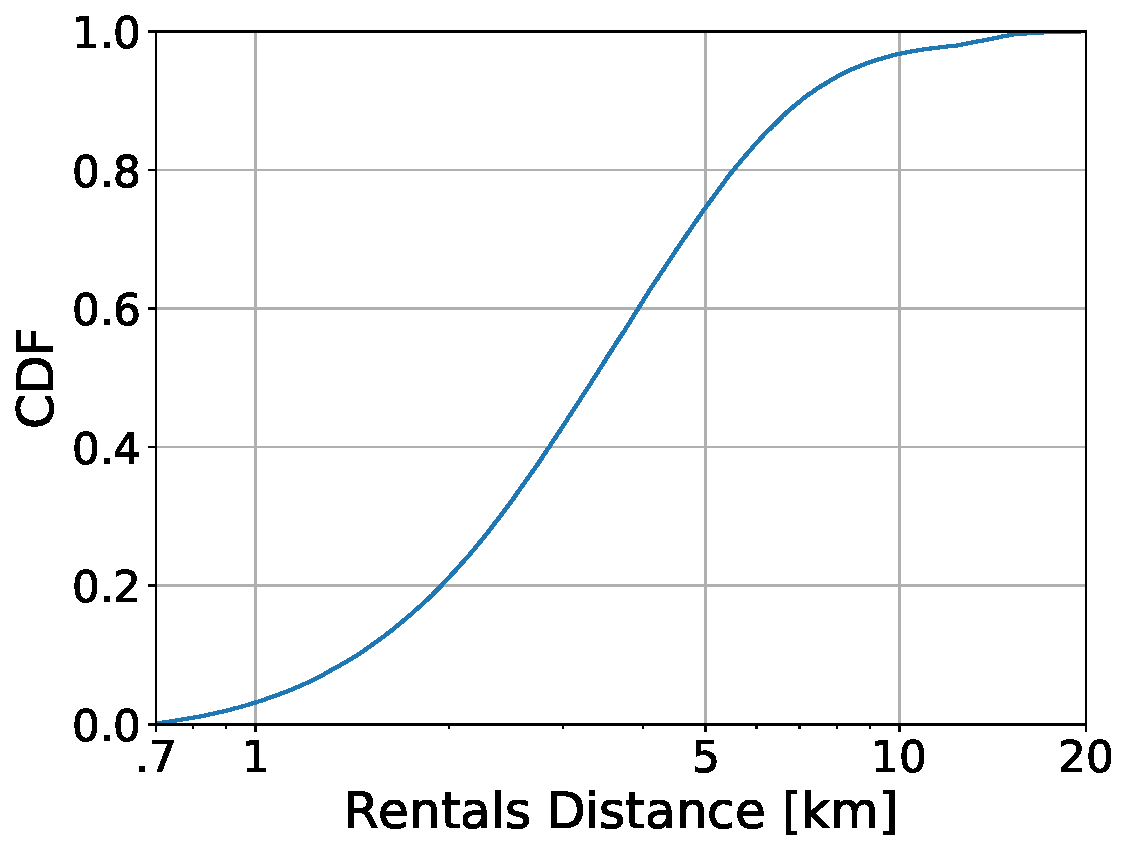
\includegraphics[width=0.45\columnwidth]{figures/CDF_distance.pdf}
        }
        \subfigure[CDF of parking durations. X-axis is logarithmic, and limited to 2 days.]{
            \label{fig:cdf_duration}
            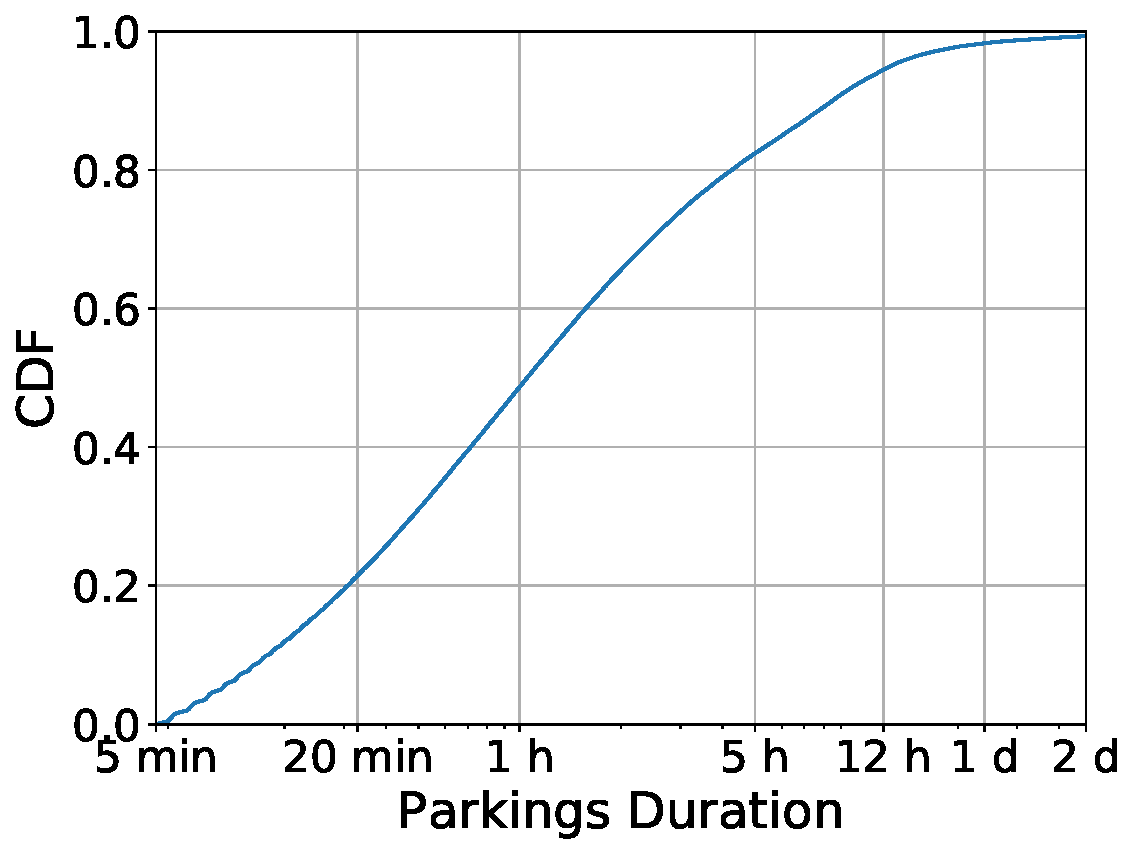
\includegraphics[width=0.45\columnwidth]{figures/CDF_duration.pdf}
        }
        \caption{Characteristics of the trips in our \DIFdelbeginFL \DIFdelFL{dataset}\DIFdelendFL \DIFaddbeginFL \DIFaddFL{data-set}\DIFaddendFL .}
        \label{}
\end{figure}


Next, we analyse how parking habits are different in the city area. For this, we divide the service operative area using a grid of squared zones of 500x500 meters, obtaining 261 zones covering Turin.
For each zone, we compute the total number of parkings recorded \DIFdelbegin \DIFdel{, the sum of all the parking duration, }\DIFdelend and the average parking time.




Fig. \ref{fig:hm_max-parking} shows the heatmap of the total number of parkings in each city zone. The warmer the colour is, the more frequently cars are parked here. The hot areas correspond to the city centre which exhibits the highest number of parkings. Customers rely on car sharing for travelling and moving downtown, a working area full of shops and restaurants. The zones with more parkings are close to the train stations, where 47 parking events per day are observed on average.
On the contrary, few parkings are observed in the suburbs (down to less than 1 event per day), where people likely return home in the evening~\cite{UMAP}. 

Fig. \ref{fig:hm_avg-time} shows the heatmap of the average parking time for each zone. Peaks are on borders of the operative area, where parking events last more than 24 hours. Few cars reach these peripheries  and rest unused for long time (see also rightmost part of Fig. \ref{fig:cdf_duration}). The lower values are registered in the downtown, where cars stay parked only for 85 minutes on average.

The large spread of parking density and duration challenges the decision on where to place charging stations. Indeed, if placed in areas where cars are frequently parked but for short time (e.g., city centre), batteries would get little charge. If placed in areas where few cars stay parked for long time (e.g., suburbs),  cars will be fully charged cars but occupying the station for long time.

\begin{figure}[th]
    \centering     %%% not \center
        \subfigure[Number of Parkings.]
            {
            \label{fig:hm_max-parking}
            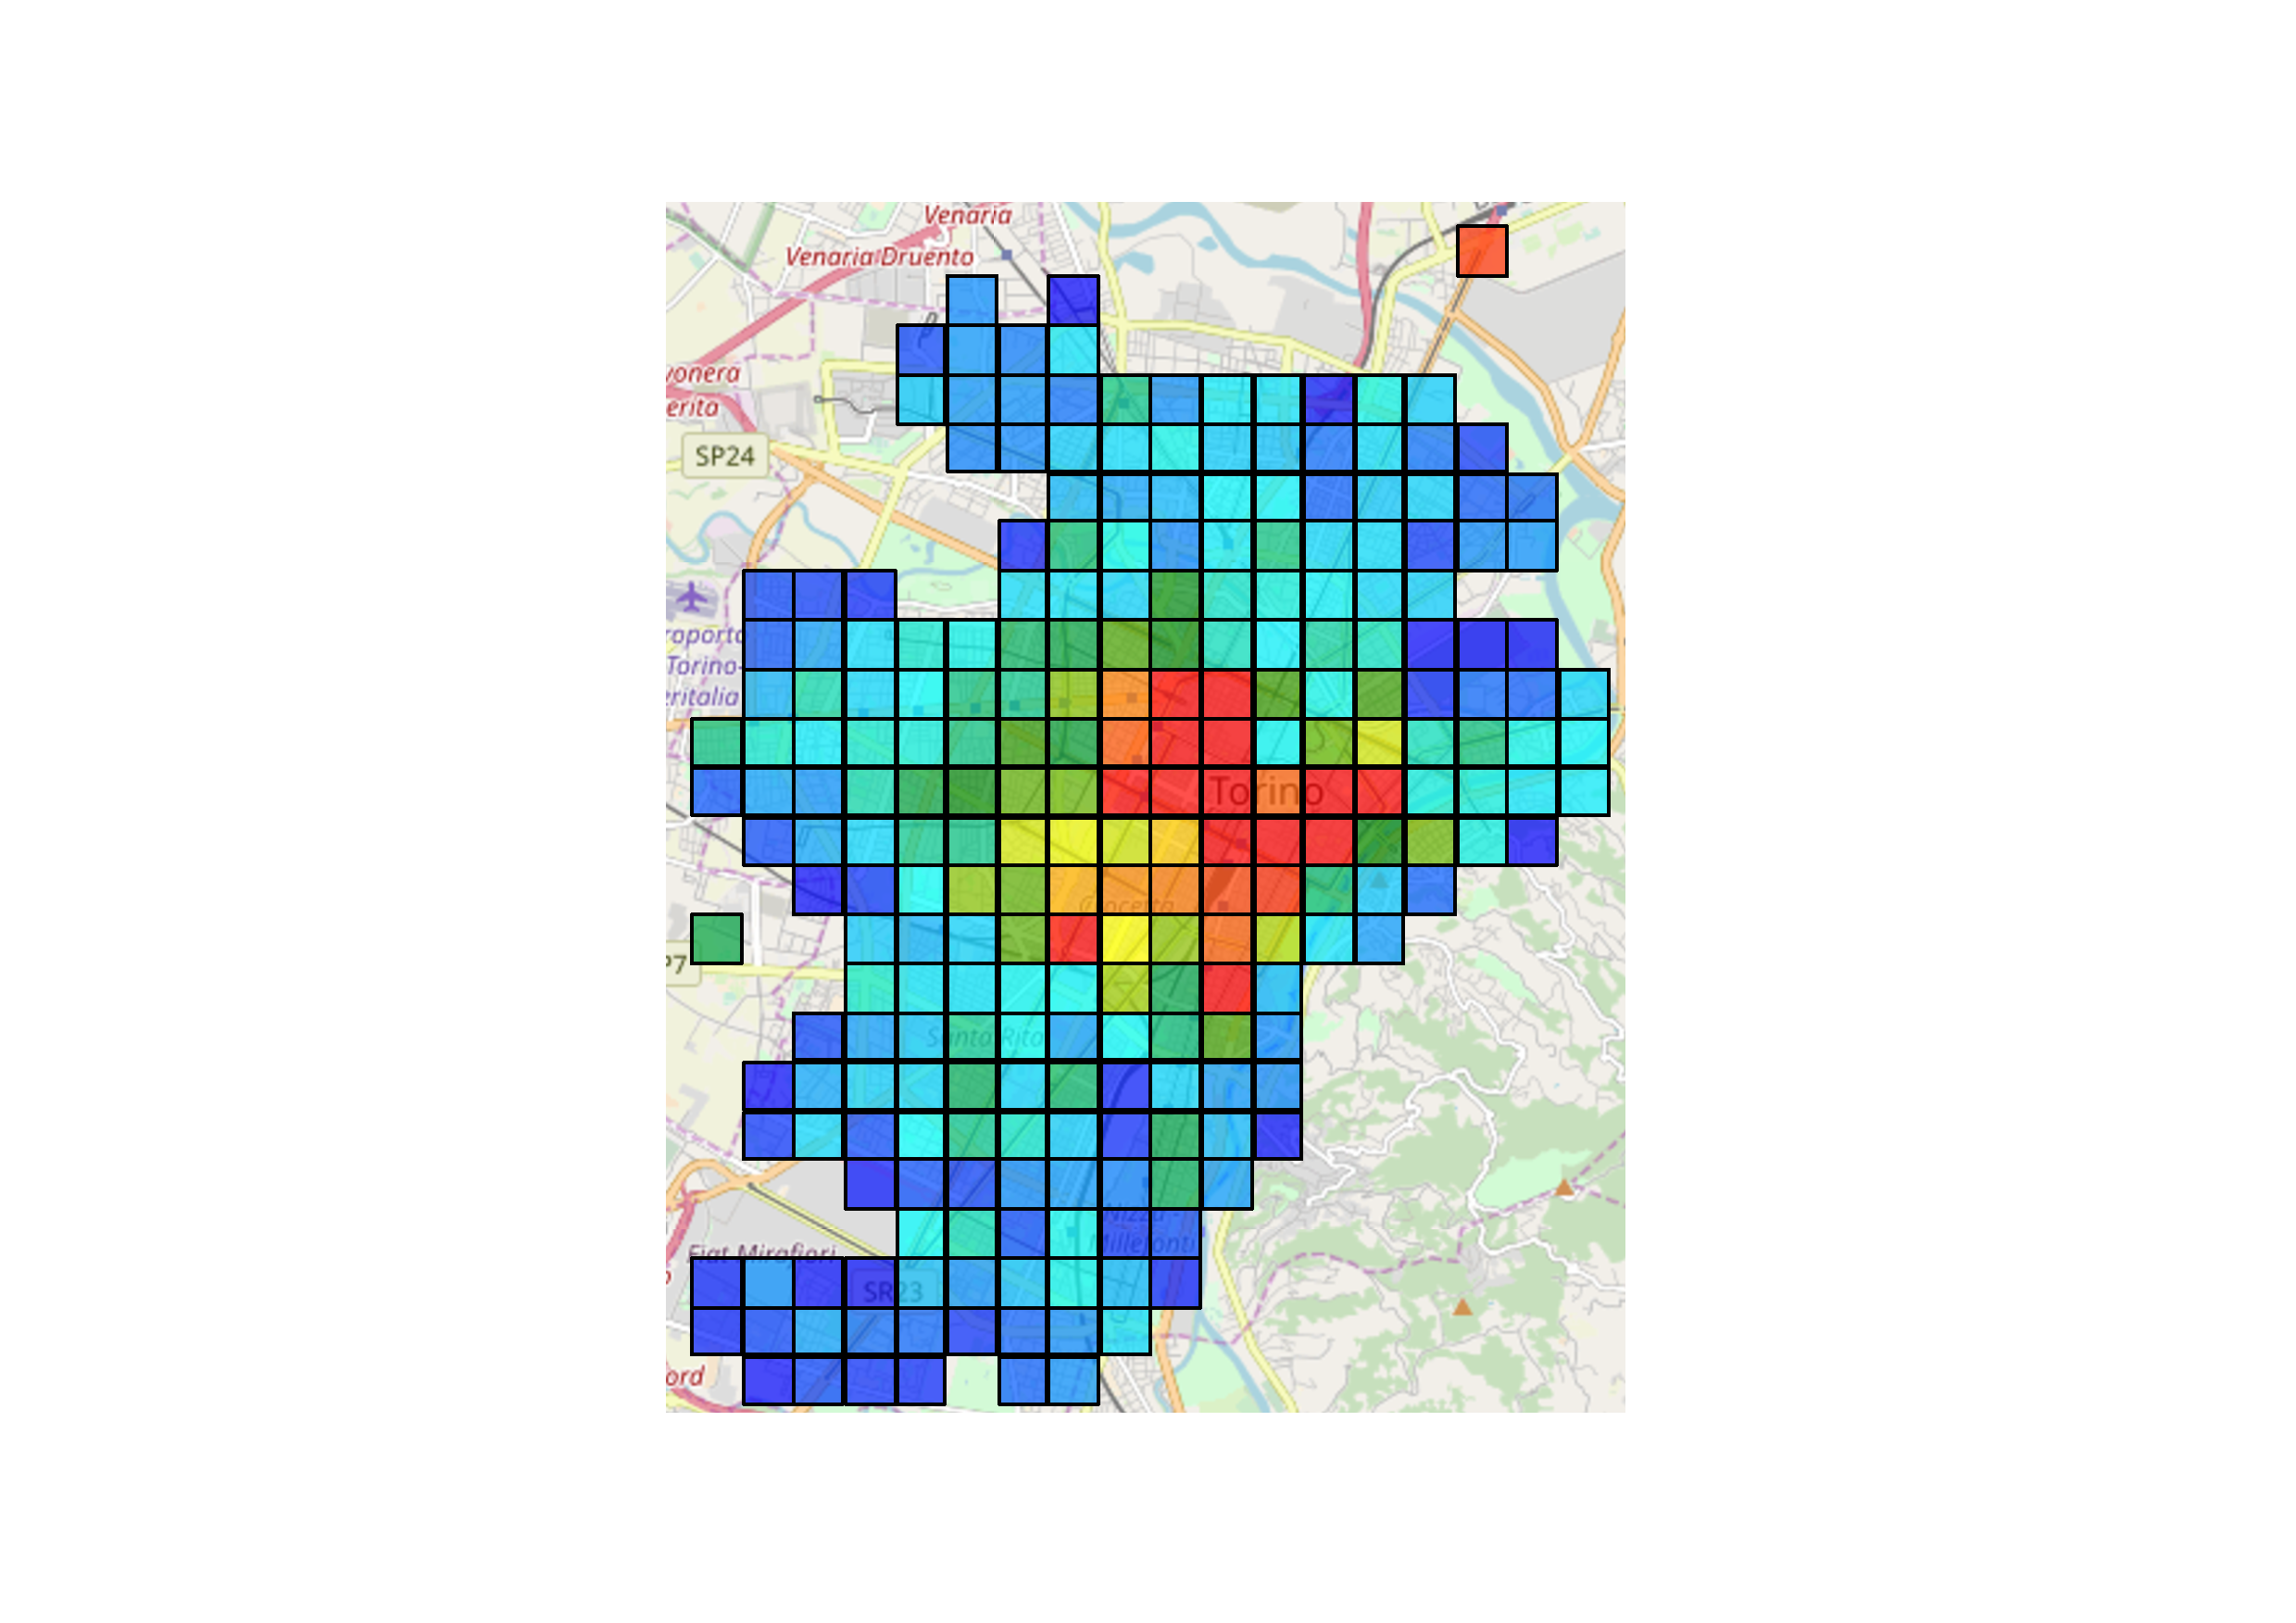
\includegraphics[width=0.35\columnwidth]{figures/Torino_NParkings.pdf}
            }
        \subfigure[Average Parking Time.]
            {
            \label{fig:hm_avg-time}
            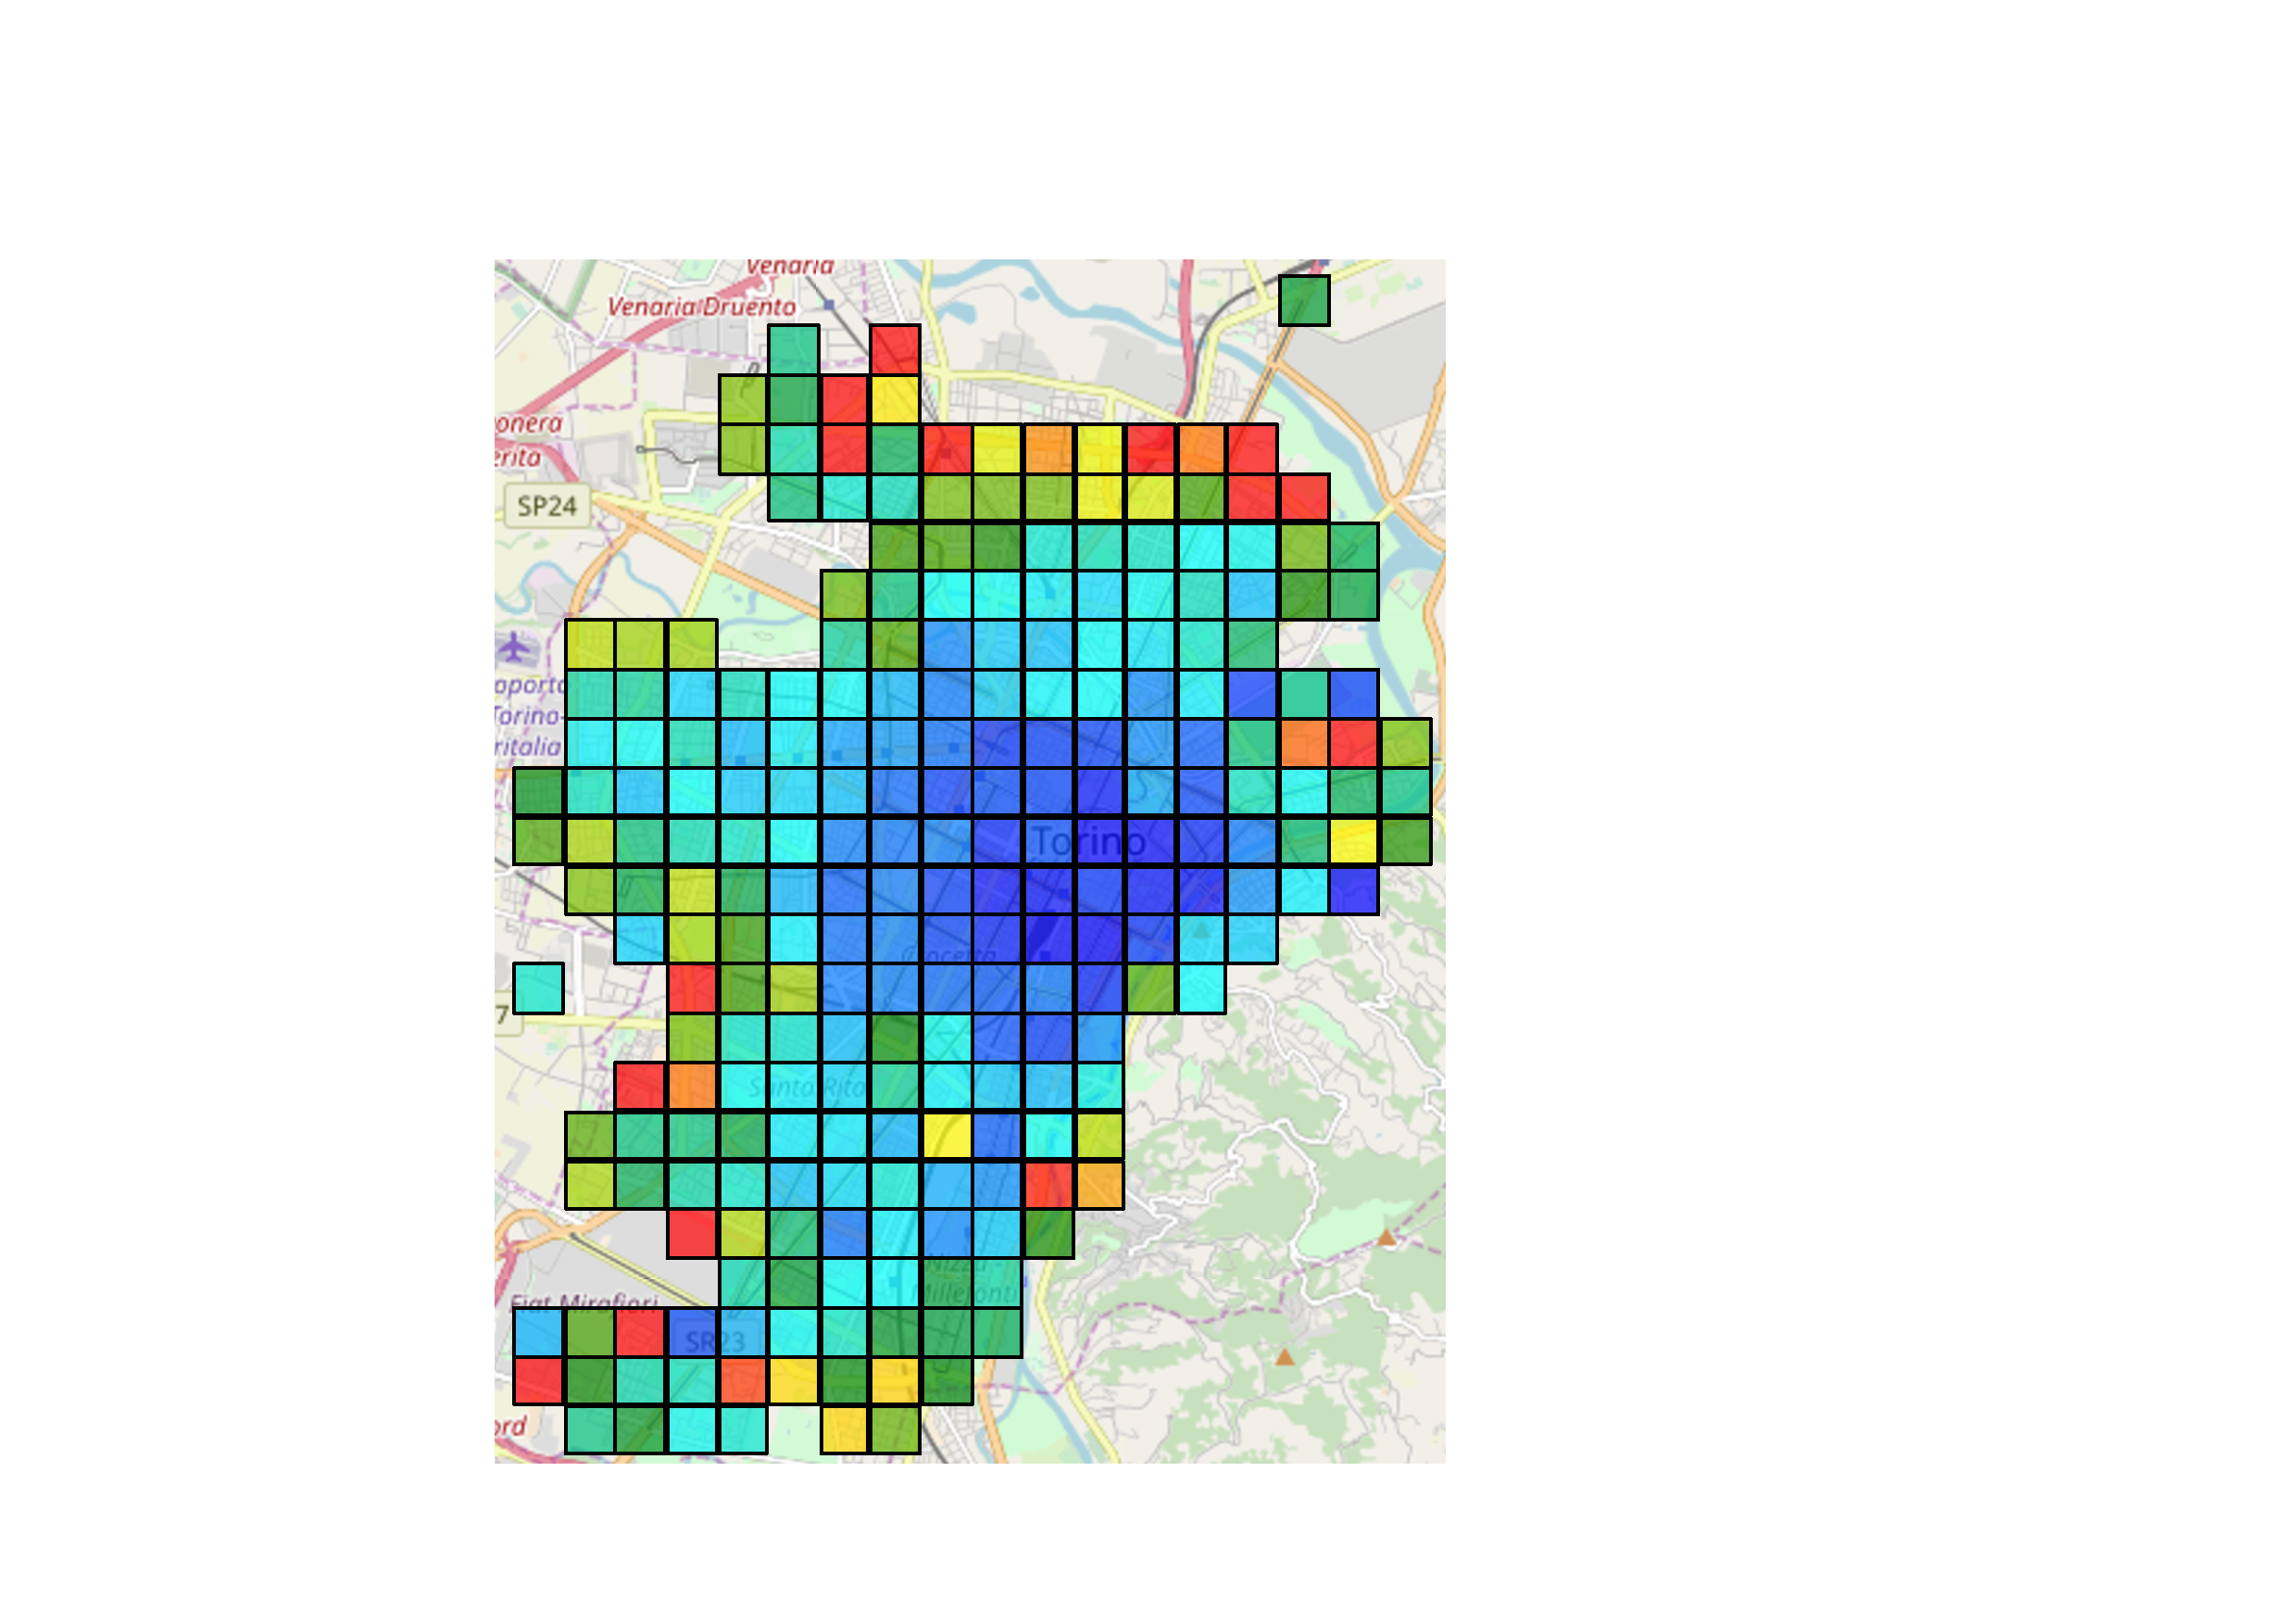
\includegraphics[width=0.35\columnwidth]{figures/Torino_AvgTime.pdf}
            }
    	\caption{Heatmaps showing (a) number of parkings per zone  and (b) average parking time per zone. Warmer areas have larger values. }
    	\label{fig:data_car}
\end{figure}
\section{Electric car sharing simulator}
\label{sec:Modelling}

Our goal is to study different design choices for electric car sharing systems, based on collected data. For this, we developed a flexible event-based simulator that allows us to compare different algorithms and tune  parameters while collecting metrics of interests.


We simulate a fixed fleet of electric cars. Each car is characterised by its parking location, and the current status of battery charge. 
The simulator takes as input \DIFdelbegin \DIFdel{a }\DIFdelend \DIFaddbegin \DIFadd{the }\DIFaddend pre-recorded \DIFdelbegin \DIFdel{trace of rentals}\DIFdelend \DIFaddbegin \DIFadd{data-set of rentals, i.e., the trace, }\DIFaddend characterised by the start and end time, and initial and final geographic coordinates. For simplicity, space is divided into 261 zones of 500\,x\,500\,m each (as explained in Section \ref{sec:data}). 


\subsection{Trace event processing}

Each recorded rental reflects a mobility interest of \DIFaddbegin \DIFadd{a }\DIFaddend customer, i.e., a desired trip.
\DIFdelbegin \DIFdel{The simulator process events in order of time. 
}\DIFdelend \DIFaddbegin \DIFadd{In more details, each trip $i \in \mathcal{I}$  is characterised by its start and end time, $t_{s}(i)$ and $t_{e}(i)$, and origin and destination coordinates, $o(i)$ and $d(i)$. We associate each position to the zone $O(i)=zone(o(i))$ and $D(i)=zone(d(i))$. We assume a charging station $cs$, composed of $k$ poles, can be placed at the centre of a given zone $z\in \mathcal{Z}$, so either $cs(z)=1$ if the station is present, or $cs(z)=0$ otherwise. $N=\sum_{z\in \mathcal{Z}}cs(z)$ is the total number of zones equipped with charging stations, with $K=N\cdot k$ the total number of poles.
}\DIFaddend 

\DIFaddbegin \DIFadd{We have a set $\mathcal{A}$ of cars, where each car $a\in \mathcal{A}$ at time $t$ is characterised by its position $p(a,t)$, its zone $P(a,t)=zone(p(a,t))$, and the residual battery capacity $c(a,t)\in[0,C]$, with $C$ being the maximum nominal capacity.
}

\DIFadd{The simulator processes each rental event $i$ in temporal order. 
}\DIFaddend When a car rental start event \DIFaddbegin \DIFadd{$i$ at time $t=t_{s}(i)$ }\DIFaddend is processed, the (simulated) customer looks for a car in the initial position zone \DIFaddbegin \DIFadd{$O(i)$}\DIFaddend . If cars are present, the customer rents the most charged one, independently whether the car is at a pole being charged or not.\footnote{We choose this policy because people are worried about vehicle range~\cite{RangeAnxiety}.}
%DIF < However, this hypothesis helps the charging stations to be emptied when cars are charged: for a more realistic approach, real customer behavour should be better evaluate in future work.
\DIFaddbegin \DIFadd{In formulas, we get a car $\bar{a} \in \mathcal{A}$ such that:
}

$$
\DIFadd{c(\bar{a},t) \geq c(\hat{a},t)\ \forall \hat{a} \in \argmin_{a \in A} }{ \DIFadd{dist(O(i), P(a,t))}}\DIFadd{.
}$$


\DIFaddend If no car is present, the customer walks to the closest zone containing an available car, mimicking the normal behaviour of FFCS customers that look for the closest car to rent on their smartphones.
A car rental end event is then scheduled using the trace final time \DIFdelbegin \DIFdel{and location.
}%DIFDELCMD < 

%DIFDELCMD < %%%
\DIFdel{When a car }\DIFdelend \DIFaddbegin \DIFadd{$t_{e}(i)$ and desired destination location $d(i)$. 
When car $a$ }\DIFaddend rental end event \DIFaddbegin \DIFadd{at time $t_{e}(i)$ }\DIFaddend is processed, the customer returns the car \DIFaddbegin \DIFadd{in  $p(a,t_{e}(i))$, chosen according to the behaviour described in the next paragraph}\DIFaddend . The simulator updates the battery charge status by consuming an amount of power proportional to the trip distance\DIFdelbegin \DIFdel{. }\DIFdelend \DIFaddbegin \DIFadd{:
}

$$
	\DIFadd{c(a,t_{e}(i)) =  \max{(c(a,t_{s}(i)) - Energy(p(a,t_{s}(i)), p(a,t_{e}(i))))} 
}$$

\DIFadd{with $Energy(\cdot)$ that models the energy necessary to go from the car origin $p(a,t_{s}(i))$ to the car destination $p(a,t_{e}(i))$.
Here we consider $Energy(\cdot)$ to be dependent only on the two positions and proportional to their distance, but more complicated functions can be easily implemented.
}

\DIFaddend In case the battery level drops below 0 \DIFaddbegin \DIFadd{($c(a,t_{e}(i)) = 0$)}\DIFaddend , the trip \DIFaddbegin \DIFadd{$i$ }\DIFaddend is declared {\it infeasible}. The discharged car still performs further trips, all marked as infeasible, until it reaches a charging station.\DIFaddbegin \footnote{\DIFadd{This is instrumental to give an exhausted car the chance to recover energy.}}
\DIFaddend 

Depending from the return policy, the customer may connect the car to a charging pole. We investigate the following return policies:
 \begin{itemize} 
	\item{\it Free Floating}: the customer opportunistically connects the car to a charging pole if and only if it is available (present and free) in the final desired zone \DIFaddbegin \DIFadd{$D(i)$}\DIFaddend ;
	\item{\it Needed}: cars are connected to a pole only when the battery level at the end of the rental goes below a minimum percentage threshold $\alpha$\DIFaddbegin \DIFadd{, i.e., $(c(a,t_{s}(i)) - Energy(p(a,t_{s}(i)), d(i))) / C\leq  \alpha $}\DIFaddend . This implies the customer can be \textit{rerouted} to the closest zone  with an available free charging pole, if none exists in the desired final zone \DIFaddbegin \DIFadd{$d(i)$}\DIFaddend ; 
	\item{\it Hybrid}: the customers follow the Needed policy, but voluntarily connect to a charging pole -- if available -- in the desired ending zone, whatever car charge status is;
 \end{itemize} 

The \textit{Free Floating} policy never obliges the customer to bring the car far from the desired ending location, even in case battery charge is close to exhaustion. \textit{Needed} mandates to connect cars to a charge station only if battery runs low, thus trying to protect from battery exhaustion. \textit{Hybrid} mixes the two policies letting customers opportunistically recharge the battery whenever they park close to a charging station.

\DIFaddbegin \DIFadd{Notice that policies similar to }\emph{\DIFadd{Needed}} \DIFadd{have been introduced in~\mbox{%DIFAUXCMD
\cite{2_FlathIlgWeinhardt_2012}}%DIFAUXCMD
, where the system make the users charge the car considering the battery state of charge, the instantaneous electricity cost,  and the user's range anxiety.
}

\DIFaddend \subsection{Performance metrics and parameters}
\label{sec:metrics}

We measure the following metrics, that we identify having influence in the customers' quality of experience:
 \begin{itemize} 
	\item \textit{InfeasibleTrips\%}: percentage of infeasible trips due to completely discharged battery observed \DIFdelbegin \DIFdel{durint }\DIFdelend \DIFaddbegin \DIFadd{during }\DIFaddend the whole simulation;  
	\item \textit{Charges\%}: percentage of trips where the \DIFdelbegin \DIFdel{customers have to connect }\DIFdelend \DIFaddbegin \DIFadd{customer connects }\DIFaddend the car to a charging pole, implying the burden to plug the car;
	\item \textit{Reroutings\%}: percentage of trips where the customers are rerouted to a zone different from their original destination because they are forced to charge the car;
	\item \textit{WalkedDistance}: walked distance from the desired destination. This is considered non-zero both when the car is charged or rerouted. The walk distance when \DIFdelbegin \DIFdel{charging in a pole of }\DIFdelend \DIFaddbegin \DIFadd{returning the car to a pole in }\DIFaddend the desired final destination is considered to be 150\,m, i.e., the average distance from any point to the centre of a square of  500\,m side;
 \end{itemize} 

Infeasible trips are critical, and the system shall be engineered so that they never happen. Other performance metrics shall be minimised. 
In addition to the above metrics, the simulator collects statistics about car battery charge level, and fraction of time a battery stays under charge. 

The key design parameters that we focus on are (i) number of zones $Z$ which are equipped with a charging station; (ii) the locations of charging stations within the city; (iii) \DIFdelbegin \DIFdel{return policies customers adopt}\DIFdelend \DIFaddbegin \DIFadd{adopted return policies}\DIFaddend .

We consider the following scenario: the fleet has a constant number of cars equal to 377 (the same as observed in the trace).  Electric cars have the same nominal characteristics as the Smart ForTwo Electric Drive, i.e., $17.6\,kWh$ battery, for $135\,km$ of range, with a discharge curve that is proportional to the travelled distance ($12.9\,kWh/100\,km$).\footnote{\url{https://www.smart.com/uk/en/index/smart-electric-drive.html}} 
Charging stations have 4 low power ($2\,kW$) poles each. These are cheap to install and a good compromise between costs, power requested, and occupied road section. We model a simple linear charge profile (complete charge in 8 hours and 50 minutes in our case).
For \textit{Hybrid} and \textit{Needed} policy we set the minimum battery charge threshold, $\alpha$, equal to $25\%$. This is a precautionary approach, since the maximum travel distance is 19 km (Fig. \ref{fig:cdf_distance}), corresponding to about 14\% of the battery capacity.
At last, the initial position of the cars, only affecting the initial transient, is randomly chosen.

Our Python simulator
%, and available open-source~\cite{MicheleGithub} %\footnote{\github}
completes a single simulation including 125\,000 rentals in less than 5 seconds.\footnote{We are able to run up to 40 simulations in parallel on a 40-core Intel Xeon 
%\textsuperscript{\textregistered} Xeon\textsuperscript{\textregistered}
processor with 128~GB of RAM, running Ubuntu 16.04 OS.} To post-process generated results and extract aggregated data,  we use PySpark\footnote{\url{http://spark.apache.org/docs/latest/api/python/\#}} on a Big Data cluster of 30 nodes. 
%The full anonymised trace is also publicly available~\cite{MicheleGithub}.%\footnote{The anonymised trace is available at \trace}.


\section{Strategies for charging station placement}\label{sec:placement}

The main objective of this paper is to assess what is the best charging station placement. Assuming that we have $Z$ zones and $N$ charging stations, there are ${N}\choose{Z}$ possible placement solutions, which makes it prohibitive to find exhaustively the optimal solution. For this reason we evaluate different approaches. The first one uses domain knowledge acquired by characterising the data about current usage to propose heuristics. The second instead, uses two different data-driven simulation-based optimisers.

\subsection{Heuristic placements}

Each zone $z$ is assigned a likelihood $l_z$. We greedily choose the top $Z$ zones, according to three likelihood definitions:
 \begin{itemize} 
\item{\it Average parking time}: $l_z$ is the average parking duration in $z$ as measured in the trace; the stations will be located in the areas where cars stay parked the longest time, hence with more probability to fill-up the battery during a charging event;
\item{\it Total number of parkings}: $l_z$ is the total number of parking events recorded in $i$ in the trace; hence the stations will be located in the areas with more parking events. Likely, more cars will be charged;
\item{\it Random placement}: $l_z$ is an independent and identical distributed random uniform variable. As such, recharging stations result placed at random over the city area;
 \end{itemize} 
The first two heuristics are driven by the intuition to place charging stations in those zones where cars are likely to be parked for long time, or frequently. The latter is presented as a baseline for comparison. Referring again to Fig.~\ref{fig:hm_max-parking} and~\ref{fig:hm_avg-time}, the charging stations will be located in the zones with warmer colours, respectively for total number of parkings and average parking time policy.

\subsection{Simulation based advanced optimisation strategies}\label{sec:optmizers}

Given the complexity of the optimisation problem and the humongous space of possible solution, we investigate the adoption of meta-heuristics, a class of global optimisation algorithms~\cite{RA09}. These algorithms explore the space of possible solutions in smart ways, looking for better solutions while avoiding getting trapped into local minima.

In our case, the evaluation of a solution requires the simulation of two months of rentals, which is performed in approximately 5 seconds on a high-end machine. It is then important to consider that we have limited resources in the choice of meta-heuristics to consider. 
The class of optimisation problems where the number of solutions (i.e., fitness evaluations) have to be limited as much as possible lies in the so called expensive-optimisation~\cite{RA09,FP09}. 
%This optimisation concerns simulation-based problems in which computational analyses are expensive in terms of time and resources \cite{RA09}.
%This field demands fast algorithms for solving optimisation problems using as few function evaluations  as possible. 
In the literature, there are several architectures and algorithms suitable for global optimisation in tough numerical problems~\cite{FP09}, with direct-search class algorithms that explicitly target expensive-optimisation problems. %Several nature-based techniques have been developed. In particular, genetic algorithms~\cite{GO89}, proved to work well when dealing with discrete variables functions. 

In our work, we \DIFdelbegin \DIFdel{consdier }\DIFdelend \DIFaddbegin \DIFadd{consider }\DIFaddend a simple local-search algorithm based on a hill-climb method, and a more complex and powerful genetic algorithm. We explicitly design both algorithms with the perspective of reducing the number of simulations. Both are implemented in our open-source tools~\cite{MicheleGithub}.

We consider the single-objective case, i.e., algorithms have to minimise a single fitness function $f$ defined as follow:
%reported Eq.~\ref{eq:fitness}.
% \begin{equation} 
$$f = M \cdot InfeasibileTrips\% + WalkedDistance$$
% \label{eq:fitness}
% \end{equation}

As commonly done in linear programming, $M$ is a number big enough to make the first addend always larger than the second.
In this way, \textit{InfeasibleTrips\%} has to be minimised first. Secondly, the algorithms starts minimising the \textit{WalkedDistance\%}. In a nutshell, we look for solutions that make all trips feasible, and only then we target the customers discomfort, i.e., reducing the walked distance. 
As we will better show in the next section, reducing \textit{WalkedDistance} will naturally help in reducing also \textit{Charges\%} and \textit{Reroutings\%}. Indeed, in its definition, the walked distance weights both these metrics.


\subsubsection{Hill-climbing local search}

Hill-climbing methods belong to the family of local search algorithms and are a popular choice because they are fast, simple to implement, and requires limited computational resources. They are iterative algorithms that start with an arbitrary solution, then attempt to find a better solution by making incremental changes to the solution. If the change produces a better solution, it is selected as current solution. Incremental changes are then made to the latter, until no further improvements can be found.
For non-convex problems, like the one here faced, these methods will find only local optima, from which it would be impossible to escape. 
Local optima are not necessarily the globally best possible solution.

Our hill-climbing algorithm is very similar to the coordinate descent version~\cite{CoordinateDescent}.
We start from the best configuration found among the three heuristics.
At each iteration, the algorithm randomly picks a charging station, and moves it in a empty neighbouring zone, i.e., north, south, east and west adjacent zones. All other charging stations are left untouched. If there is a direction of improvement, we perform a line search along the best direction, i.e., we keep moving the same station along the same direction. When no improvement is possible, we take another charging station at random, and try to move it as before.
When no improvement is found after a complete cycle of all charging station, a local minimum is reached and the algorithm exits. We also stop the local search after a maximum number of visited solutions.

In our implementation, we check multiple neighbours in parallel. Moreover, the algorithm keeps memory of all tested configurations, hence avoiding useless and expensive simulations. For details see~\cite{MicheleGithub}. 
\DIFdelbegin %DIFDELCMD < 

%DIFDELCMD < %%%
\DIFdelend In our experiments, on average the optimisation reaches convergence within 1\,500 maximum tested solutions. 

%Coordinate descent successively minimizes along coordinate directions to find the minimum of a function. 
%Coordinate descent is based on the idea that the minimization of a multivariable function can be achieved by minimizing it along one direction at a time, i.e., solving univariate (or at least much simpler) optimization problems in a loop

\subsubsection{Genetic optimiser}

Genetic algorithms are a particular class of evolutionary algorithms inspired by the natural evolution~\cite{GO89}. They are known to work well when dealing with discrete variable functions, as in our case. 

Genetic algorithms start creating a random population of a given number of individuals. In our case, each individual corresponds to a random placement of charging stations. A mating pool is created from the initial population, then the offspring is generated by crossover and mutation operations. Crossover mixes the genes from different individuals picked at random, i.e., a child is created from the union of the genes of both parents. To keep the number of genes (i.e., charging stations) constant, random genes are removed so that at the end $Z$ are left.
Mutation instead moves a single charging station in a random empty zone. During crossover operation, some genes may mutate with low probability ($P\{mutation\}=0.02$ in our case).

The presence of clones is avoided by the algorithm, which discards the copies, thus encouraging the exploration of the search space and saving precious resources. The algorithm estimates the quality of each new individual computing the fitness function $f$, i.e., by running an entire simulation.

As by natural selection, the best individuals survive to the next generation, while the worst individuals are suppressed. 
The optimisation loop continues until the maximum number of generations is reached (200 in our case).

If the diversity of available genes, i.e., the total number of distinct charging stations in the whole population, decreases too much without improvements, we increase the population genetic diversity by increasing the mutation probability ($P\{mutation\}=0.2$ in this case). This randomises the evolution. More details about the algorithm can be found in our open-source implementation~\cite{MicheleGithub}.

The algorithm is amenably suitable for parallel implementation since the fitness of each individual belonging to a specific generation can be analysed separately from the others. Another advantage of genetic algorithms is the widespread exploration of the solution space, while local search algorithms tend to explore only limited portion of the space.

In our experiments, we set the initial population to 100, with 50 new individuals created at each generation by crossover. Most of the optimisations ended within 100 generations, i.e., 5\,000 overall solutions are evaluated through simulation.
\section{Impact of heuristic placements and return policies}
\label{sec:freefloating}

 %Indeed, this solution will be our baseline to evaluate the return policies.




\subsection{Impact of heuristic charging station placements}

In this first set of experiments we evaluate which heuristic placement performs better.
Firstly, for each heuristic we consider the simple opportunistic \textit{Free Floating} car return policy, i.e., customers always return the car in the desired zone, and connect it to a charging pole if available. The goal is to check if this simple return mechanism is sustainable with electric cars, and gauge the impact of the three different heuristics for the charging station placement.

Fig.~\ref{fig:deathsVsZones_algorithm} shows the performance in terms of infeasible trip percentage versus an increasing percentage of charging zones, ranging from  1\% to 30\%. In Turin, this corresponds to install from 2 to 78 charging stations overall \DIFaddbegin \DIFadd{(reported in the top x-axis)}\DIFaddend .
We observe notably different performances. First, the average parking time placement policy (\textit{Avg time}) performs the worst, with still 6\% of infeasible trips even when  more than 25\% of zones are equipped with charging stations. Even a simple random placement performs better (\textit{Mean rnd}, obtained as the average of 10 independent instances). The total number of parkings placement (\textit{Num parking}) reaches about 2\% of infeasible trips at 10\% coverage, reaching self-sustainability when more than 20\% of zones are equipped (no infeasible trips).

\begin{figure}[ht]
	\centering
	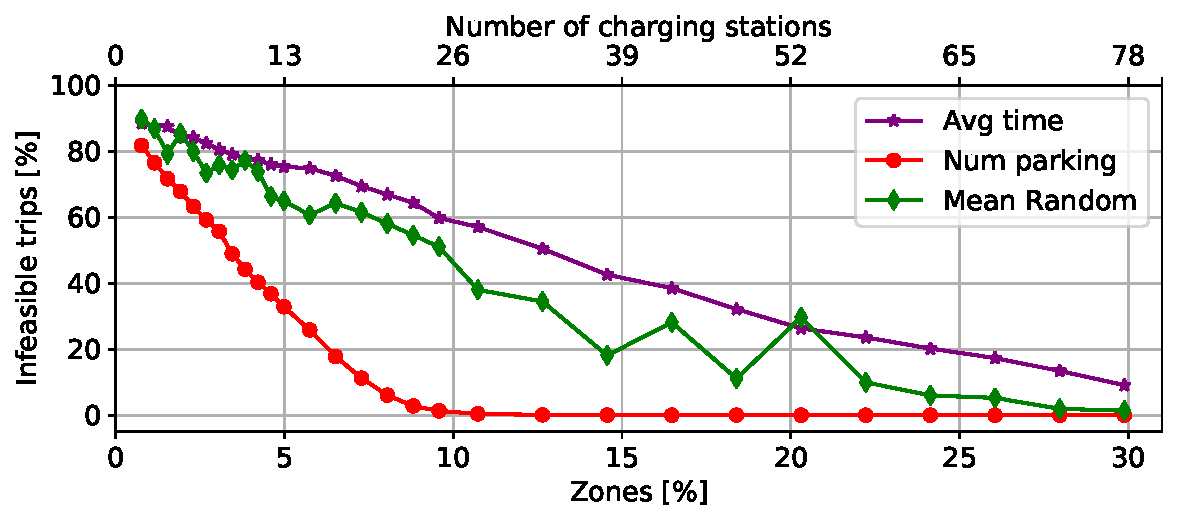
\includegraphics[width=0.9\columnwidth]{figures/Torino_FF_deaths_probs.pdf}
	\caption{Percentage of unfeasible trips as function of charging stations (percentage and number of city zones), for the different heuristic placements.}
	\label{fig:deathsVsZones_algorithm}
\end{figure}

\begin{figure}[ht]
	\centering
	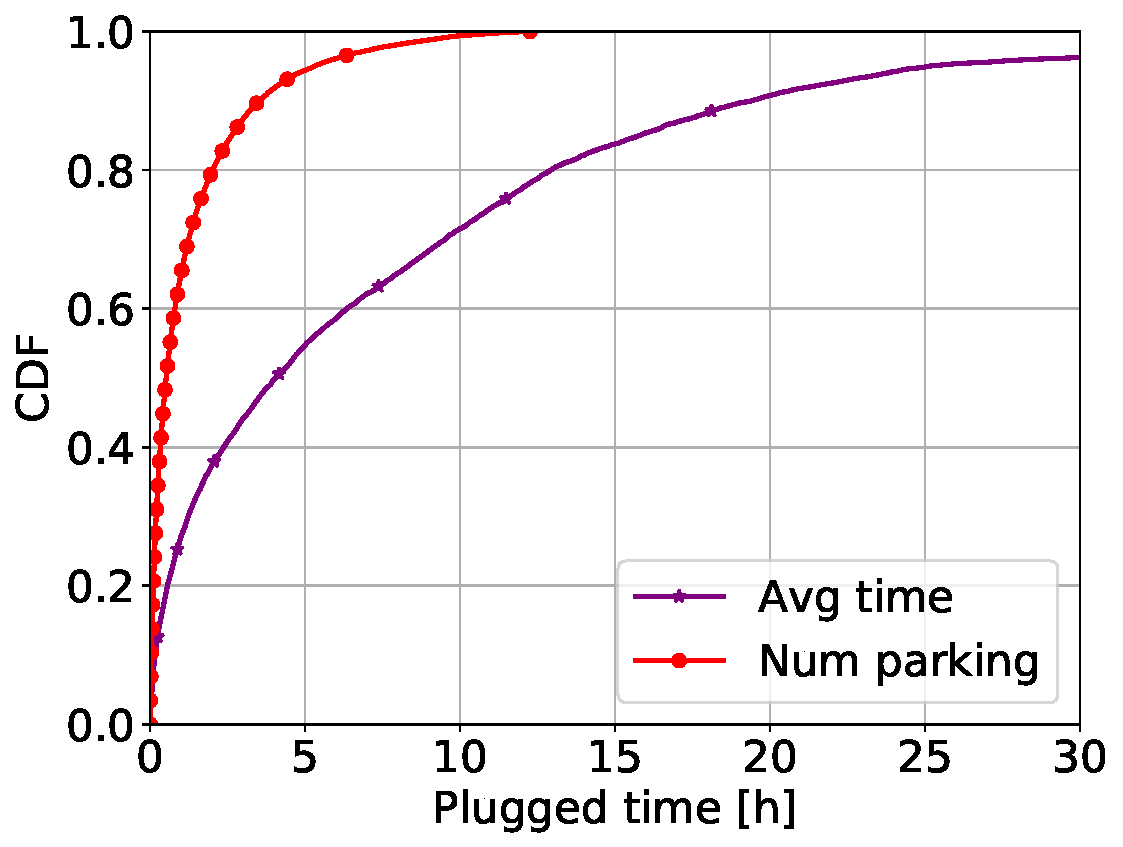
\includegraphics[width=0.5\columnwidth]{figures/CDF_parking_time_per_algorithm.pdf}
	\caption{CDF of the time spent by a car at a charging station (Z=40), for \textit{Num parking} and \textit{Avg time} placement algorithms. }
		\label{fig:CDF_parking_time_per_algorithm}
\end{figure}

The intuition of why such a striking difference is given by the different properties of areas where the heuristics place charging stations. \textit{Avg time} placement favours peripheral zones where few trips ends, and where cars stay parked for long time (see Fig. \ref{fig:hm_avg-time}). On the contrary, \textit{Num parking} favours city centre areas, where cars frequently are parked for short time (see Fig. \ref{fig:hm_max-parking}). Indeed, in the whole simulation, for $Z=40$ ($\approx 15\%$ of zones), only 7\,430 charges have been recorded for \textit{Avg time}, compared with 47\,628 charges of the \textit{Num parking}.
Even if plugged time is shorter, the \textit{Num parking} policy allows the cars to charge the (little) energy consumed during the (short) trips.
Moreover, as shown in Fig. \ref{fig:CDF_parking_time_per_algorithm} the \textit{Avg time} placement generates much longer plugged times, often much longer than the time needed for a full charge. Therefore, many cars occupy the charging poles when they are already charged, preventing other cars to use those poles and increasing the number of infeasible trips. 

In a nutshell the best approach among these three heuristics is to place charging stations in the central areas, in which the parkings last less but are more frequent. For this reason, we will use the \textit{Num parking} placement algorithm as best heuristic for the remaining of the paper.



\subsection{Impact of return policy}

We now investigate the impact of the three different return policies. We quantify the implications of forcing customers to return the car to a different zone than the desired one, when the battery is below a critical level (i.e., below the percentage threshold $\alpha=25\%$ of full battery capacity).

We focus again on the infeasible trip percentage with respect to the charging station coverage.
Fig. \ref{fig:deathsVsZones_policy} shows results, with \textit{Num Parking} placement. \textit{Needed} and \textit{Hybrid} policies perform much better than the opportunistic \textit{Free Floating}.
In details, \textit{Hybrid} and \textit{Needed} guarantee to successfully conclude all trips with just $Z=11$ and $Z=15$ charging zones, respectively (4.2\% and 5\% of the zones), while \textit{Free Floating} reaches this goal only at $Z=60$  (23\% of zones).
In a nutshell, adopting a policy which mandates customers to charge the cars when battery level gets low drastically reduces the number of infeasible trips, even with a handful of  charging stations.

\begin{figure}[ht]
	\centering
	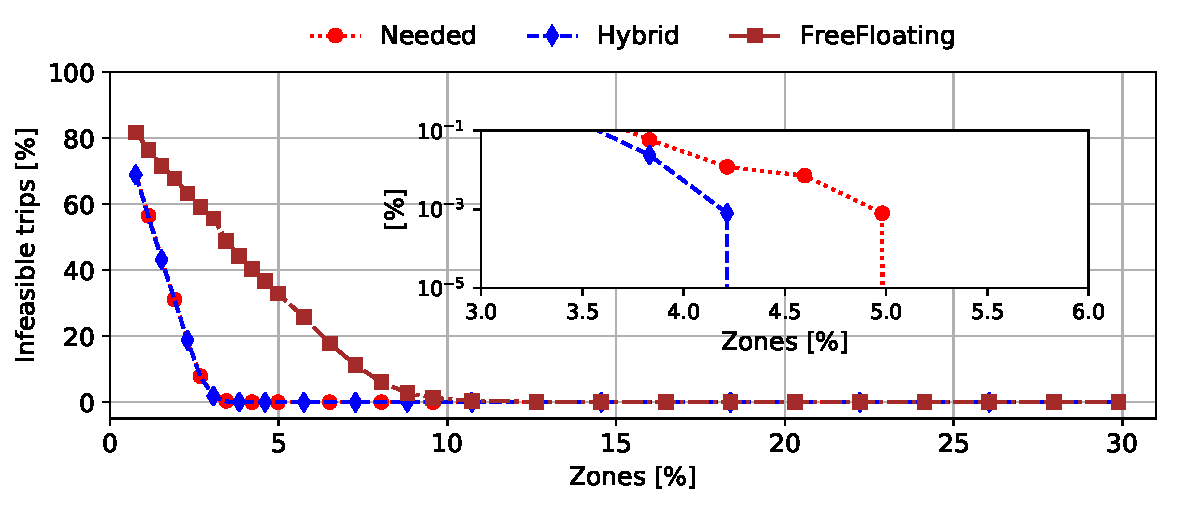
\includegraphics[width=0.95\columnwidth]{figures/Torino_H_N_FF_deaths_probs.pdf}
	\caption{Percentage of infeasible trips for different zone coverage percentage analysing the return policies. The inset highlights where the infeasible trips go to 0.}
	\label{fig:deathsVsZones_policy}
\end{figure}

\begin{figure}[ht]
    \centering     
    \subfigure[Percentage of trips ending with a charge.]
    {
        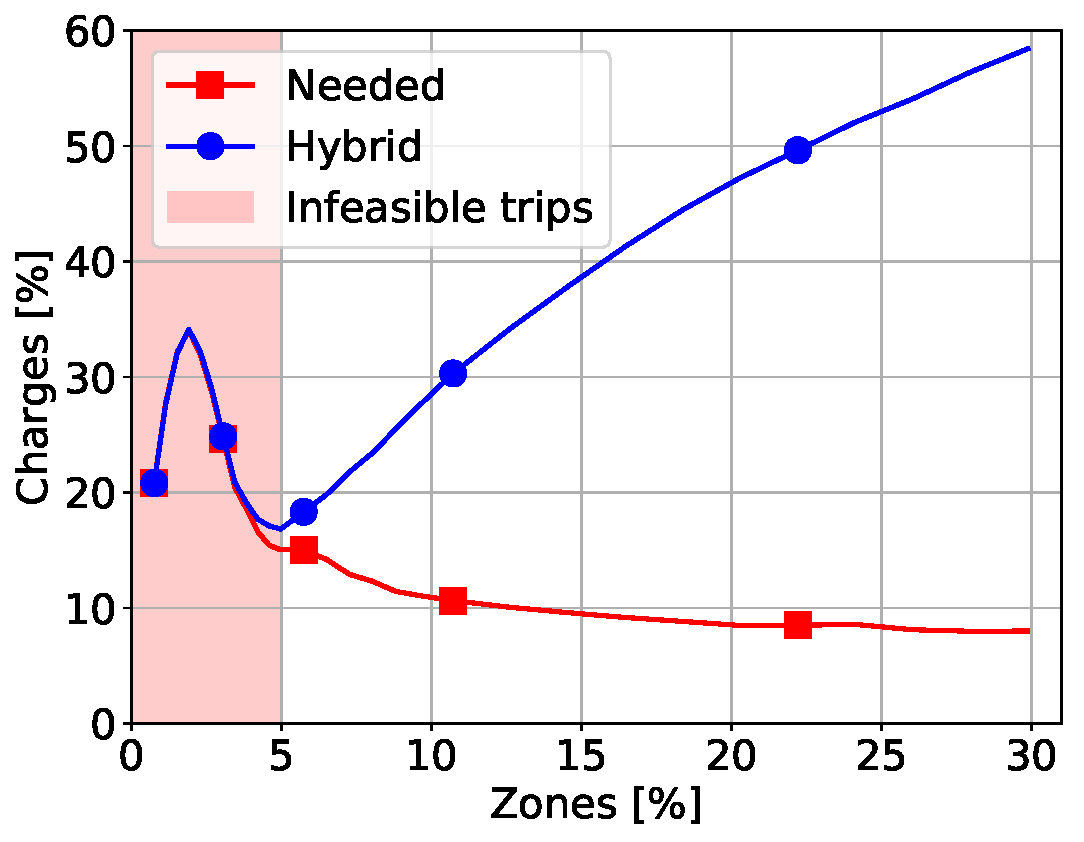
\includegraphics[width=0.45\textwidth]{figures/Taormina_Torino_AmountRechargePerc.pdf}
        \label{fig:recharge_perc}
    }
    \subfigure[Rerouted trips percentage.]
    {
        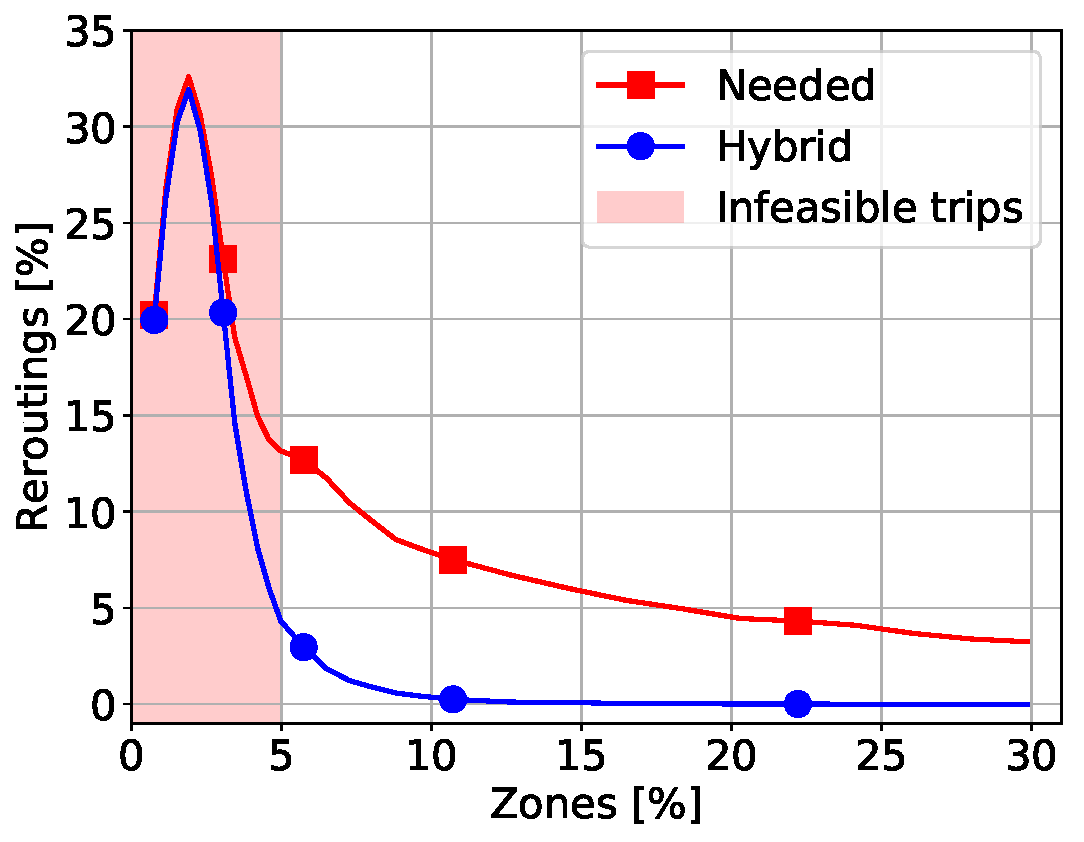
\includegraphics[width=0.45\textwidth]{figures/Taormina_Torino_ReroutePerc.pdf}
        \label{fig:reroute_perc}
    }
    \subfigure[Walked distance, averaged over all trips.]
    {
        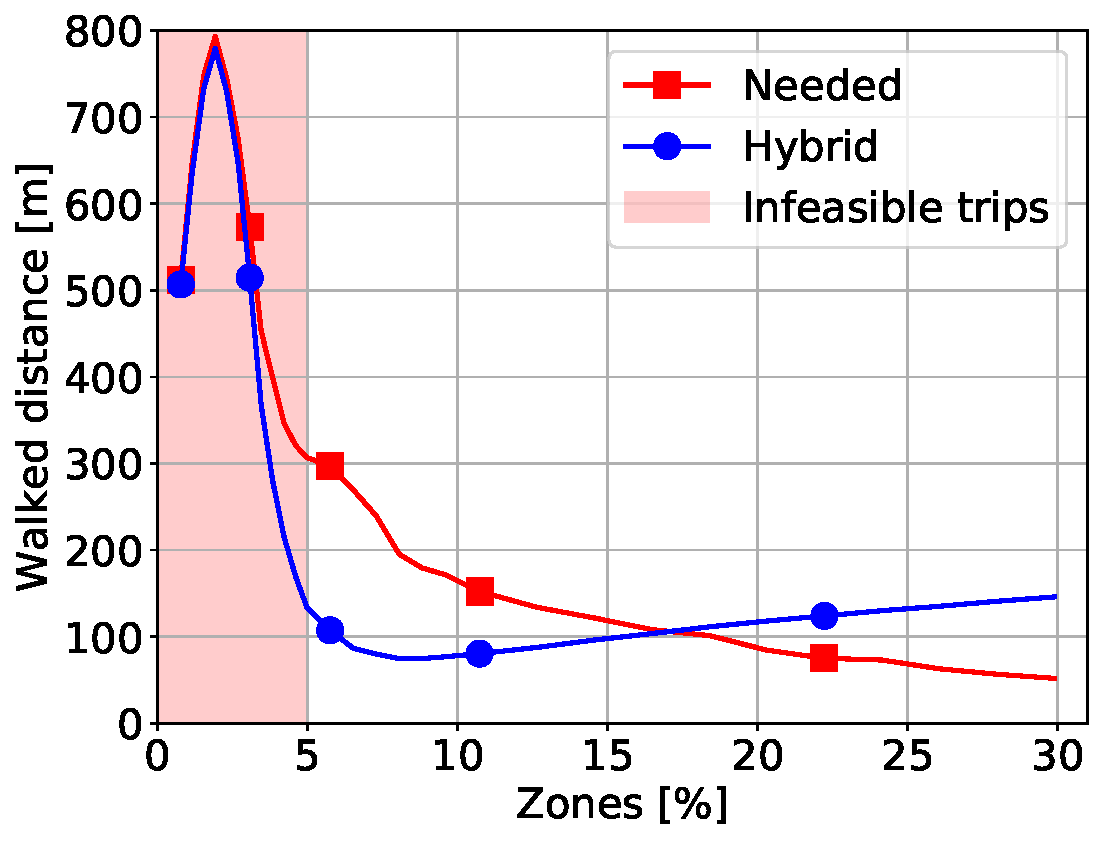
\includegraphics[width=0.45\textwidth]{figures/Taormina_Torino_TravelWithPenlaty.pdf}
        \label{fig:global_weighted_distance}
    }

    \caption{Metrics of interests when comparing Hybrid and Needed return policy (Max parking placement adopted).}
    \label{}
\end{figure}

\subsubsection{Customers' discomfort}
%questa e' una subsection della scelta della policy, non una a parte

Forcing customers to charge batteries, even at cost or rerouting them has clearly an impact on their comfort. Indeed, forcing a customer to park in a charging station can be annoying, because of the burden of reach the charging station, and losing time to plug to and unplug the car from the pole. Even worse, rerouting customers to the closest zone for charging increases the distances they have to walk to reach the desired destination. 

Fig. \ref{fig:recharge_perc} reports the percentage of trips that end by charging the car. Shaded area highlights the infeasible region, where the lack of charging zones create artefacts. Focusing on the feasible region instead, the two curves start with similar values, but then they diverge. Interestingly, the percentage of charges decreases for the \textit{Needed} policy, getting as low as 8\%. This suggests a better usage of each single charge, i.e., the battery fills up and does not need frequent charges. 
%This happens when few stations are present and all of them can be occupied. Hence some cars will not be charged despite they would need to. 
Conversely, the \textit{Hybrid} policy increases steadily the fraction of trips where customers have to plug to a pole. This because the higher $Z$, the higher the probability of ending the trip in a zone with a free charging pole.

Fig. \ref{fig:reroute_perc} represents the rerouting percentage in function of charging stations coverage.
Rerouting probability decreases as expected: the more the stations are, the more likely customers find a charging station at their desired final zone. Yet, the two policies have different performance. The \textit{Hybrid} policy is less likely to reroute customers. In fact, by opportunistically connecting the car to a charging pole if available, the average battery charge is high, thus decreasing the rerouting probability. With more than 7\% of charging zones, the percentage of rerouting is already lower than 1\% for \textit{Hybrid} policy.
In a nutshell, \textit{Hybrid} policy significantly reduces the number of times the customer has to drive to a charging station in a different zone than the desired one. However, it increases the number of times the customer parks at a charging station and has to plug the car to the pole. Therefore, one must be cautious when weighting these results and designing return policies which impact the customers' comfort. 

Whenever the system forces a customer to park the car in a charging station, customers may be routed far from their desired destination. If the charging station is not in the final destination zone, the customer has to walk by at least 500\,m to reach their final destination. Even in case the charging station is found inside the final zone, the customer will have to park at the charging station, instead of the desired destination. 
For this reason, we evaluate the average distance the customers have to walk to reach their actual final destination. 
In details, when the customers suffer rerouting, we evaluate the actual distance between the charging station and the final destination. When they end in a charging zone and plug the car, we count an average distance of 150\,m. Finally, if the customers do not charge the car, we assume they arrived at their final destination directly.

Results are shown in Fig. \ref{fig:global_weighted_distance}.
Consider the feasible region. The \textit{Needed} policy exhibits a decreasing trend (from 280 m to 60 m). On the contrary, the \textit{Hybrid} policy first exhibits a decrease (minimum of 50 m at 8\% of charging zones), but then it slowly increases till it overtakes the \textit{Needed} policy. 
This is due to the fact that with few charging stations (6-15\%) the number of charges is limited ($<$ 30\%, see Fig. \ref{fig:recharge_perc}) by the availability of charging stations. Instead, when this number grow, the opportunistic \textit{Hybrid} policy 
forces the customer to walk more \DIFdelbegin \DIFdel{(}\DIFdelend \DIFaddbegin \DIFadd{times }\DIFaddend within the ending zone\DIFdelbegin \DIFdel{)}\DIFdelend .
To this extent, the \textit{Needed} policy performs better. 

Even if the values of walked distances seem very small, remember that they are averaged over all trips. Restricting to the few long walks due to rerouting (not reported for the sake of brevity), the walked distance that we observe ranges from 2\,200\,m to 1\,500\,m, with similar behaviours for the two policies. 
Recall that the charging station placement algorithm \DIFdelbegin \DIFdel{is likely placing }\DIFdelend \DIFaddbegin \DIFadd{likely places }\DIFaddend stations mainly in the city centre. Therefore, the charging stations are concentrated in a small area, so that rerouting from the suburbs significantly affects the walked distance when rerouted. This gives hope for further optimisation, as we will see in the next section.

Given the very few rerouting of the \textit{Hybrid policy}, one can envision a system which directly takes care of those very few cars that need a battery charge, i.e. by relocating vehicles. For instance less than 3 cars per day would need to be relocated with 15\% coverage or higher.

In summary, with \textit{Hybrid} policy, less than 15\% of zones guarantees all trips to be feasible, reduces the walked distance, asks for few rerouting events, at the cost of moderately high percentage of times (40\%) customers are asked to charge the battery.





\section{Meta-heuristic optimisation of the charging station placement}
\label{sec:opt}



In the previous section, we saw how the \textit{Num Parking} placement heuristic works better than the other two.
%With more than 5\% of zones, the system sustains itself, both with the \textit{Needed} and the \textit{Hybrid} return policy. 
Weighting also charges and rerouting, the \textit{Hybrid} policy shows better performances than \textit{Needed}. For this reason, in this section, we focus on the \textit{Hybrid} return policy with charging stations covering less than 15\% of the zones. We further optimise this scenario by running the meta-heuristic placement algorithms, and comparing the results with the \textit{Num Parking} placement. 
Optimisation with \textit{Needed} return policies are briefly discussed in \ref{sec:needed}, where very similar results are obtained.  

%Despite the good performances of the heuristic approach from Fig. \ref{fig:global_weighted_distance} the customer has to walk a lot when rerouted. For this reason in this section, we exploit two optimization algorithms to improve previous results. 
%We exploit the two optimization algorithms described in Sec. \ref{sec:optmizers}.
The hill-climbing local search, here abbreviated in \textit{Local Search}, uses \textit{Num Parking} placement as initial solution. The \textit{Genetic} algorithm creates a totally new solution without exploiting any previous knowledge. 
Recall that both algorithms are designed to find the best charging stations placement that guarantee 0 infeasibile trips, and to minimise the overall distance the customer has to walk to reach the final destination.


\begin{figure}[th]
    \centering     %%% not \center
    \subfigure[Percentage of infeasible trips.  Y-Axis is logarithmic.]
    {
      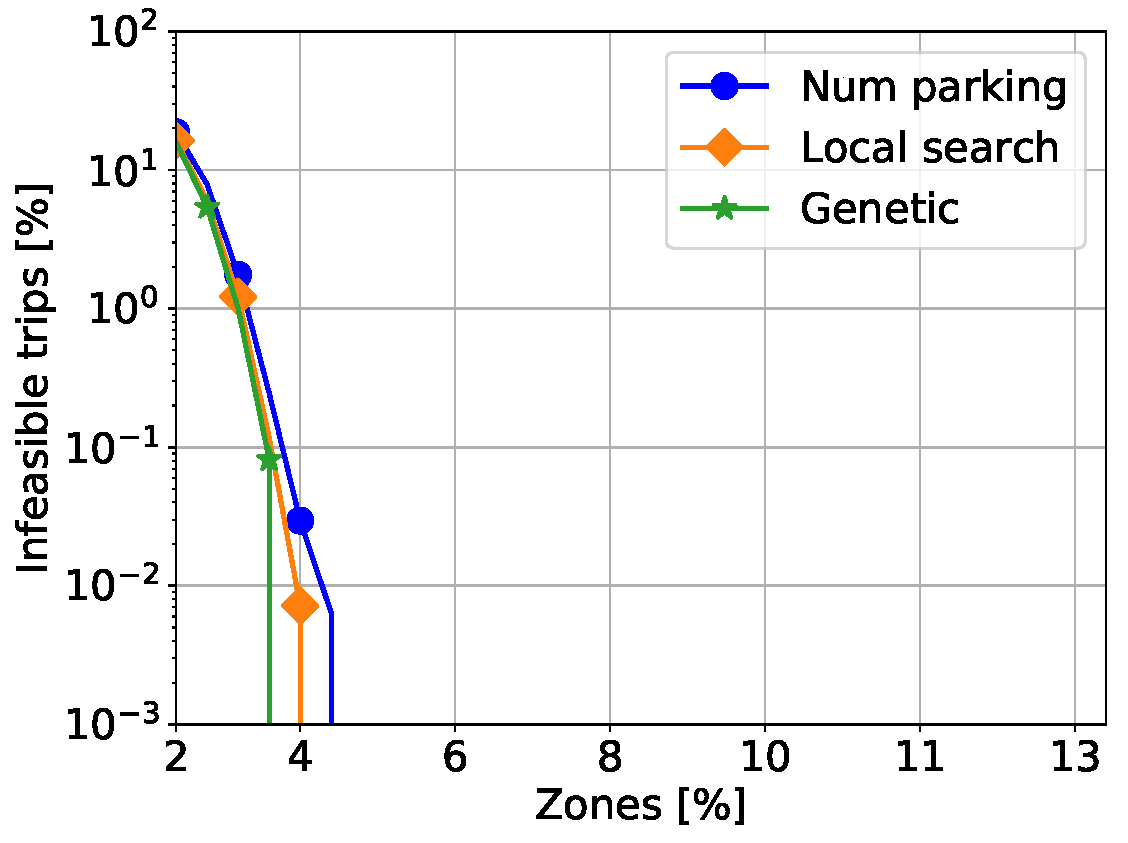
\includegraphics[width=0.45\textwidth]{figures/Hybrid_Deaths.pdf}
        \label{fig:optimized_deaths}
    }
    \subfigure[Average walked distance.]
    {
        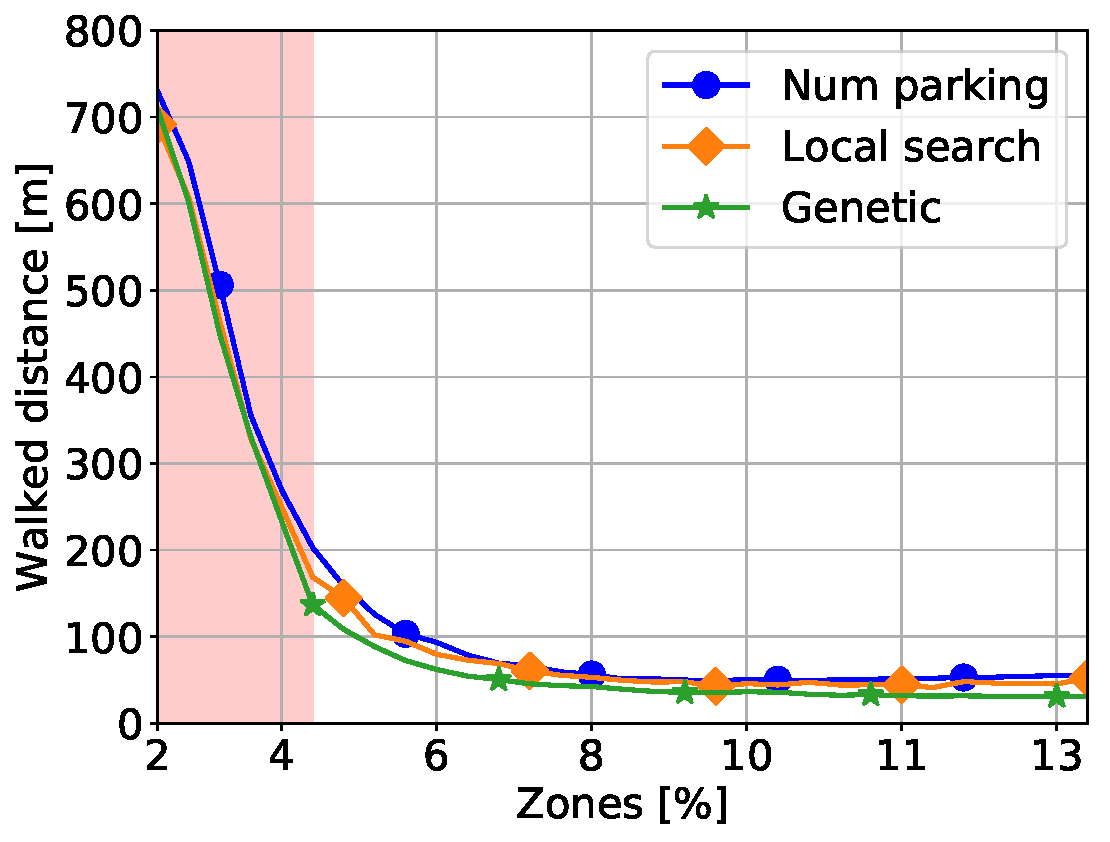
\includegraphics[width=0.45\textwidth]{figures/Hybrid_TravelWithPenlaty.pdf}
        \label{fig:optimized_penaly}
    }    
    \label{fig:optimized_metrics}
    \caption{Objective metrics to minimise in the optimisation - with \textit{Hybrid} return policy.}
\end{figure}


\begin{figure}[th]
    \centering     %%% not \center

    \subfigure[Percentage of trips ending with a charge.]
    {
        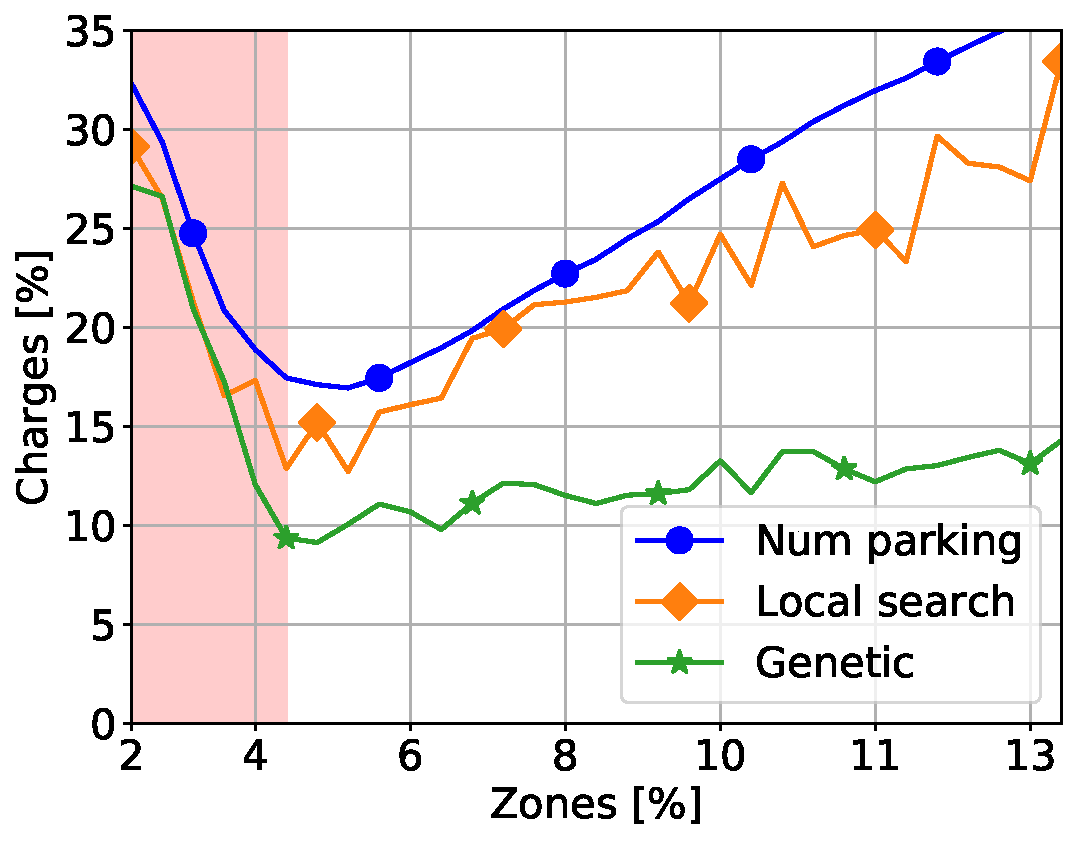
\includegraphics[width=0.45\textwidth]{figures/Hybrid_AmountRechargePerc.pdf}
        \label{fig:recharge}
    }
    \subfigure[Average state of charge.]
    {
        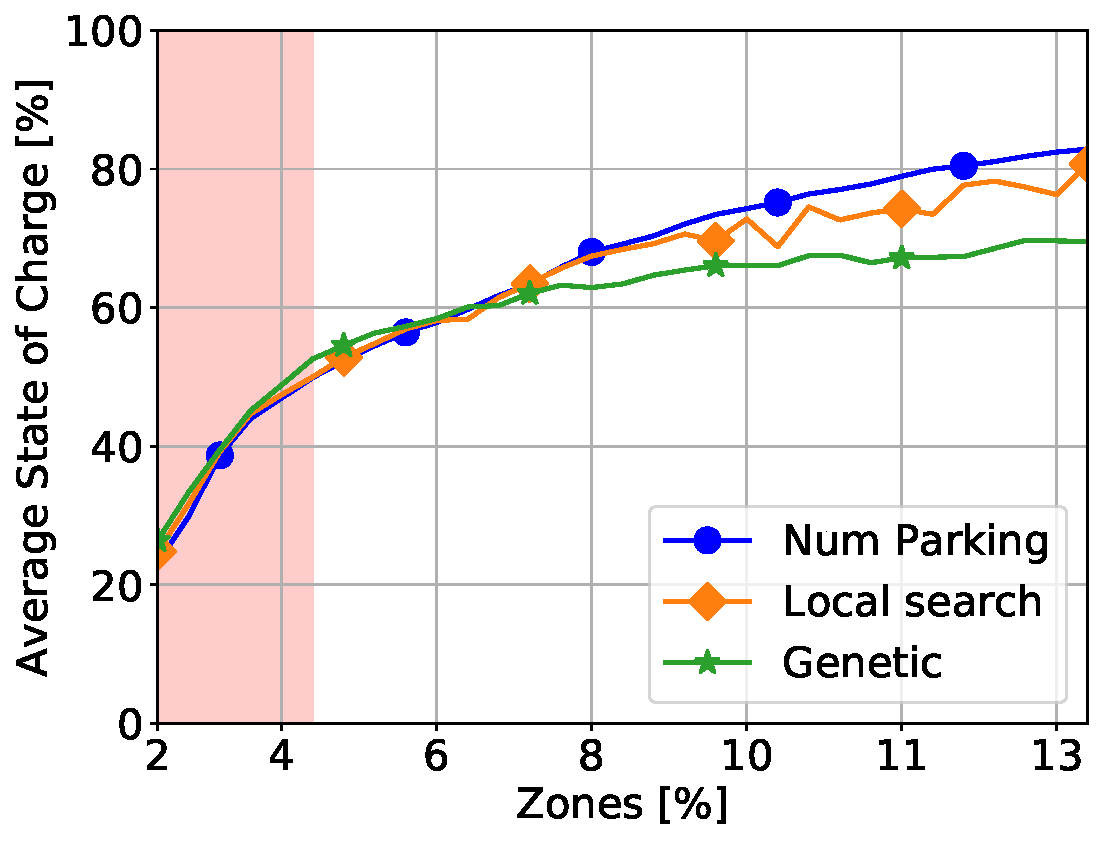
\includegraphics[width=0.45\textwidth]{figures/AvgSOC_comparison.pdf}
        \label{fig:asoc}
    }     
    \subfigure[Rerouted trips percentage.]
    {
        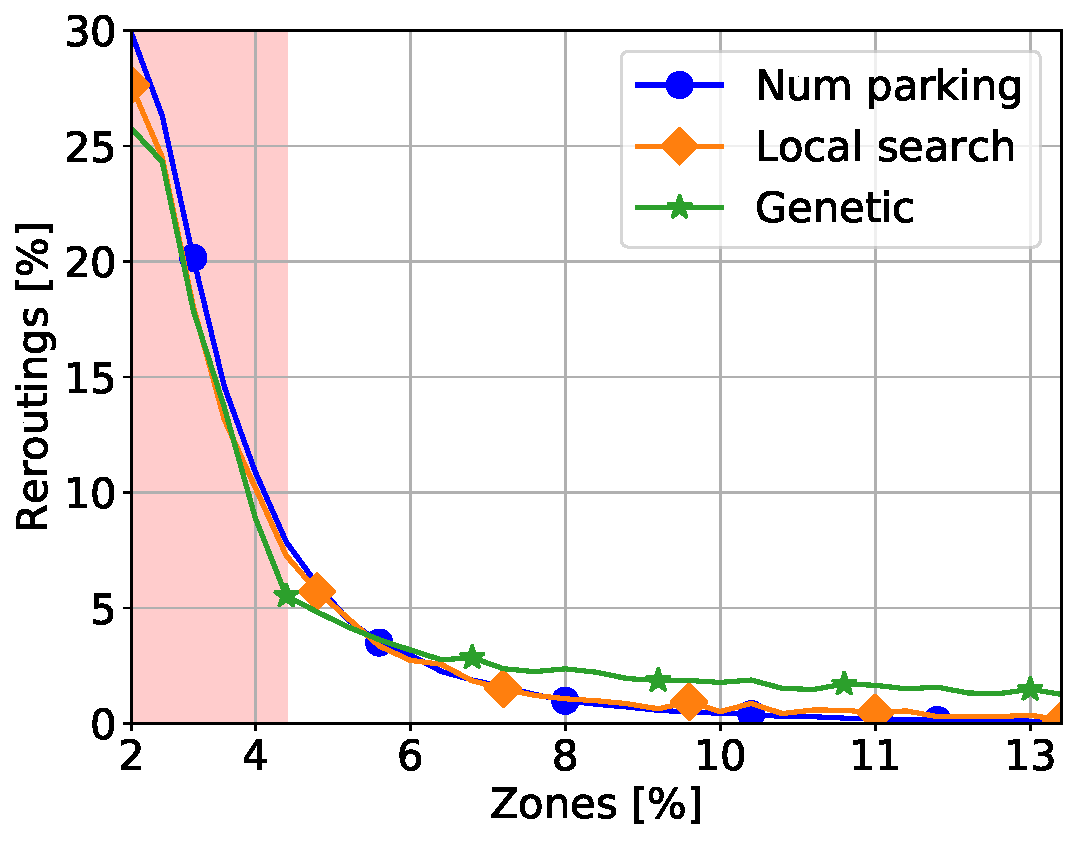
\includegraphics[width=0.45\textwidth]{figures/Hybrid_ReroutePerc.pdf}
        \label{fig:reroute}
    } 
% \subfigure[Walked distance, averaged over all trips \lv{Cambiare label asse y da Glob. w.w.d a Walked distance (vedere sezione 4.2. e 5.2 per maggiori dettagli)}]
%     {
%         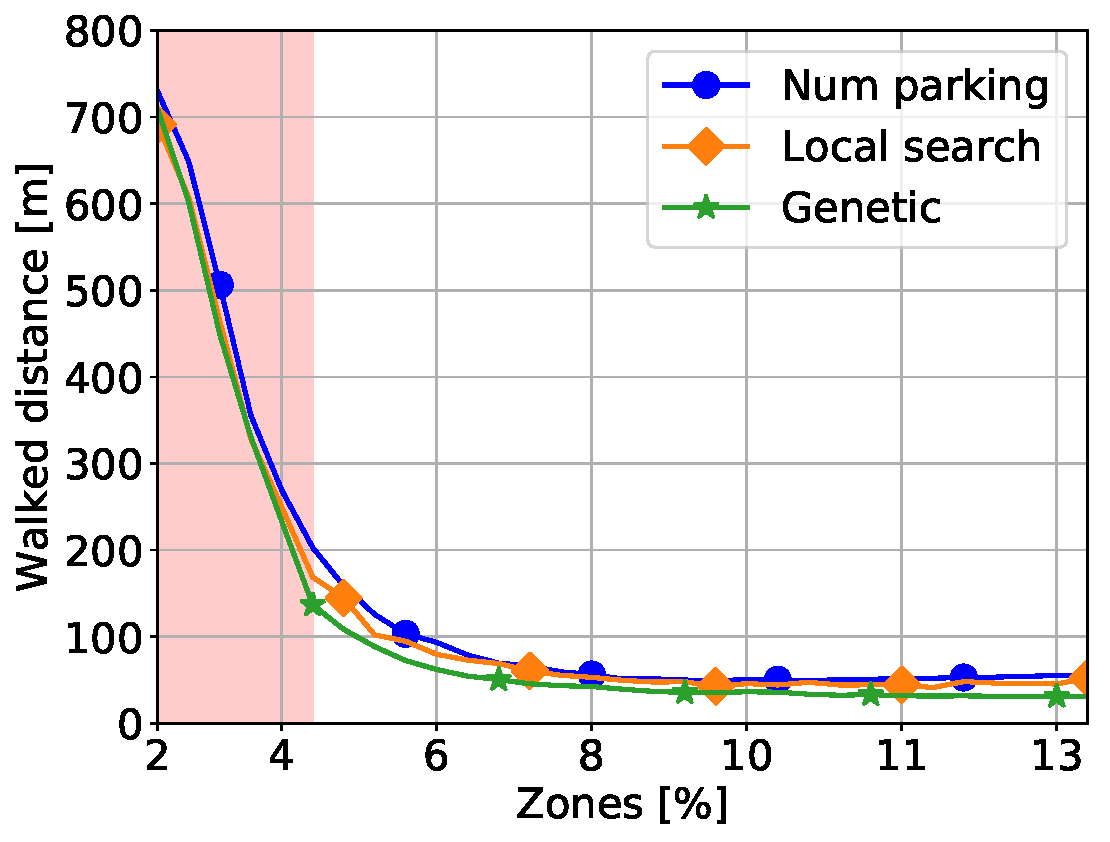
\includegraphics[width=0.3\textwidth]{figures/Hybrid_TravelWithPenlaty.pdf}
%         \label{fig:wwd}
%     }
    \subfigure[Walked distance when rerouted.]
    {
        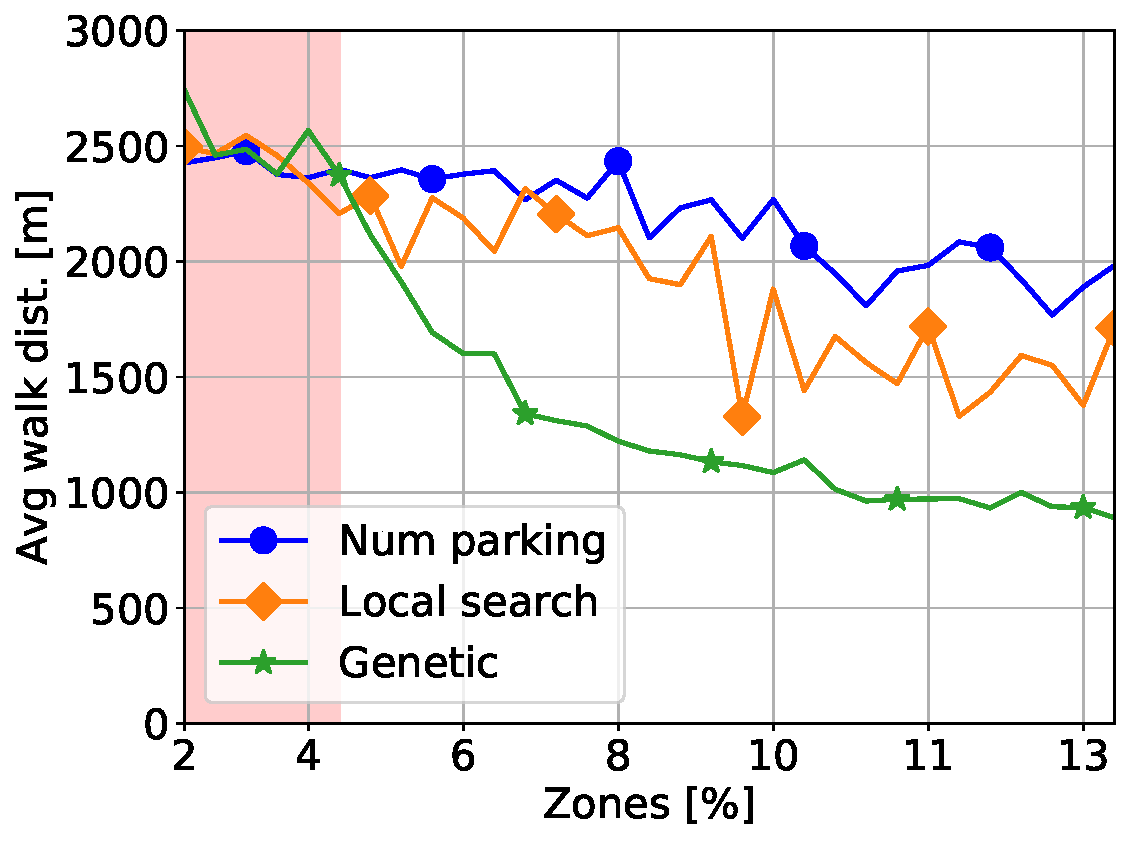
\includegraphics[width=0.45\textwidth]{figures/Hybrid_AvgWalkedDistance.pdf}
        \label{fig:awd}
    }
    \caption{\textit{Genetic} and \textit{Local Search} optimisation results for metrics of interests (\textit{Hybrid} return policy adopted). }
    \label{fig:hybrid_optimization}
\end{figure}


Fig.~\ref{fig:optimized_metrics} reports the two target metrics, for all the optimised configurations.
Firstly, in Fig.~\ref{fig:optimized_deaths} we compare the infeasible trip percentage. \textit{Num Parking} solution (blue line) has already good performance, reaching 0 with 4.2\% of the equipped zones. 
The \textit{Local Search} (orange line) and the \textit{Genetic} (green line) algorithms are able to further reduce the minimum percentage of zone to equip to guarantee no infeasible trips: 3.8\% by the \textit{Local Search}, and to 3.5\% with the \textit{Genetic} algorithm, $Z=10$ and $Z=9$ zones respectively.
%This improvements highlight that (i) \textit{Num Parking} is not the best overall placement, and (ii) local search reaches only a local optimum. 
%This improvements highlight that in the one hand, the \textit{Num Parking} solution represents a very good starting points to place charging stations. In the other hand, they prove that \textit{Num Parking} is not the best placement algorithm overall, since by using a solution not derived from it, we can achieve better performance.  
%The second objective of our optimizer is to improve the customer discomfort in terms of overall distance the customers have to walk to reach the final destination (

Fig.~\ref{fig:optimized_penaly} reports the walked distance. Focusing in the feasible region, the \textit{Genetic} algorithm confirms the best performance, reducing the distance from more than 200\,m to 136\,m when 4.2\% of the zones are equipped with charging stations, and reaching just 30\,m at 13\%. 




In Fig.~\ref{fig:hybrid_optimization} we further study the new solutions on other metrics.
Fig. \ref{fig:recharge} reports the percentage of trips ending in a charging station. The more charges are performed, the more time the customer has to spend time plugging/unplugging the car. By minimising the walked distance, we also reduce this metric, since a trip ending with a charge corresponds to 150\,m of penalty.
Here, the \textit{Local Search} follows the same trend as the \textit{Num parking} with a strong rise. The \textit{Genetic} algorithm shows much better results, from 9\% to 14\% of trips ending with a charge -- half of those found with other solutions. 
This improvement highlights the better placement of the charging stations.
Focus now on Fig. \ref{fig:asoc}, which reports the average state of charge of the car battery. 
No major difference are observed here, with all curves almost overlapping up to 7\% of the zones.

In a nutshell, the solution found by the \textit{Genetic} algorithm lets customers charge much less frequently, while keeping the average state of charge very similar. 
%Despite that in \textit{Genetic} algorithm we plug the car at most 14\% of the time, the average state of charge rise, reaching up to 70\% with 13\% of the zone.

%An other important metric to be evaluated is the percentage of rerouted trips, as the customer may be discouraged by frequent rereoutes. 
Consider next Fig. \ref{fig:reroute}, which details the percentage of reroutes. We can see how the trend is the opposite with respect to the previous ones. Here, the \textit{Genetic} optimised solution show a little higher rerouting percentage than the \textit{Num parking}. 
%Since the \textit{Local Search} and the \textit{Max parking} have similar placement, this percentage does not show particular differences with the two curves almost overlapped. Instead, 
In particular, the \textit{Genetic} algorithm 
%shows a stable reroute percentage with more than 8\% of zones, 
reaches 1.3\% of reroutes, while \textit{Num parking} decreases down to 0.2\% of reroutes. Indeed, the \textit{Genetic} algorithm places charging stations not only where most rentals ends, but also so to decrease the customers' average walked distance, i.e., in those places where likely cars are not so frequently parked but that can be quickly reached in case of rerouting.
\DIFdelbegin \DIFdel{In order to }\DIFdelend \DIFaddbegin \DIFadd{To }\DIFaddend understand the importance of this difference, in Fig.~\ref{fig:awd} we evaluate the walking distance a customer has to walk because she suffered a reroute.  
%As previously shown in Fig. \ref{fig:optimized_penaly}, the optimized algorithms show that, overall, the customer has to walk less than the \textit{Num parking} solution. In particular, Fig. \ref{fig:awd} shows that 
The \textit{Genetic} algorithm is able to push the walked distance below 1\,km, while the \textit{Local Search} generates marginal improvements.
In a nutshell, despite customers are rerouted more frequently, on average, they walk for a shorter, and  more bearable, distance.

% %3.4. usage of poles
% \lv{add plots or even just  sentence about the usage of poles? Usage of pools to show how genetic is better. Asse x numero di zone, asse y Occupazione \% delle paline, per i 3 placement}

In conclusion, a smart placement of the charging stations is better under different perspectives.  The \textit{Genetic} solution, tailored on the data of the usage behaviour, allows \DIFaddbegin \DIFadd{us }\DIFaddend to improve both the system performance, and customers' discomfort, in particular by greatly reducing the number of times they have to charge, and the distance they have to walk.


\subsection{Charging station placement visualisation}

\begin{figure}[h!]
    \centering     %%% not \center
    \subfigure[Number of Parkings.]
    {
        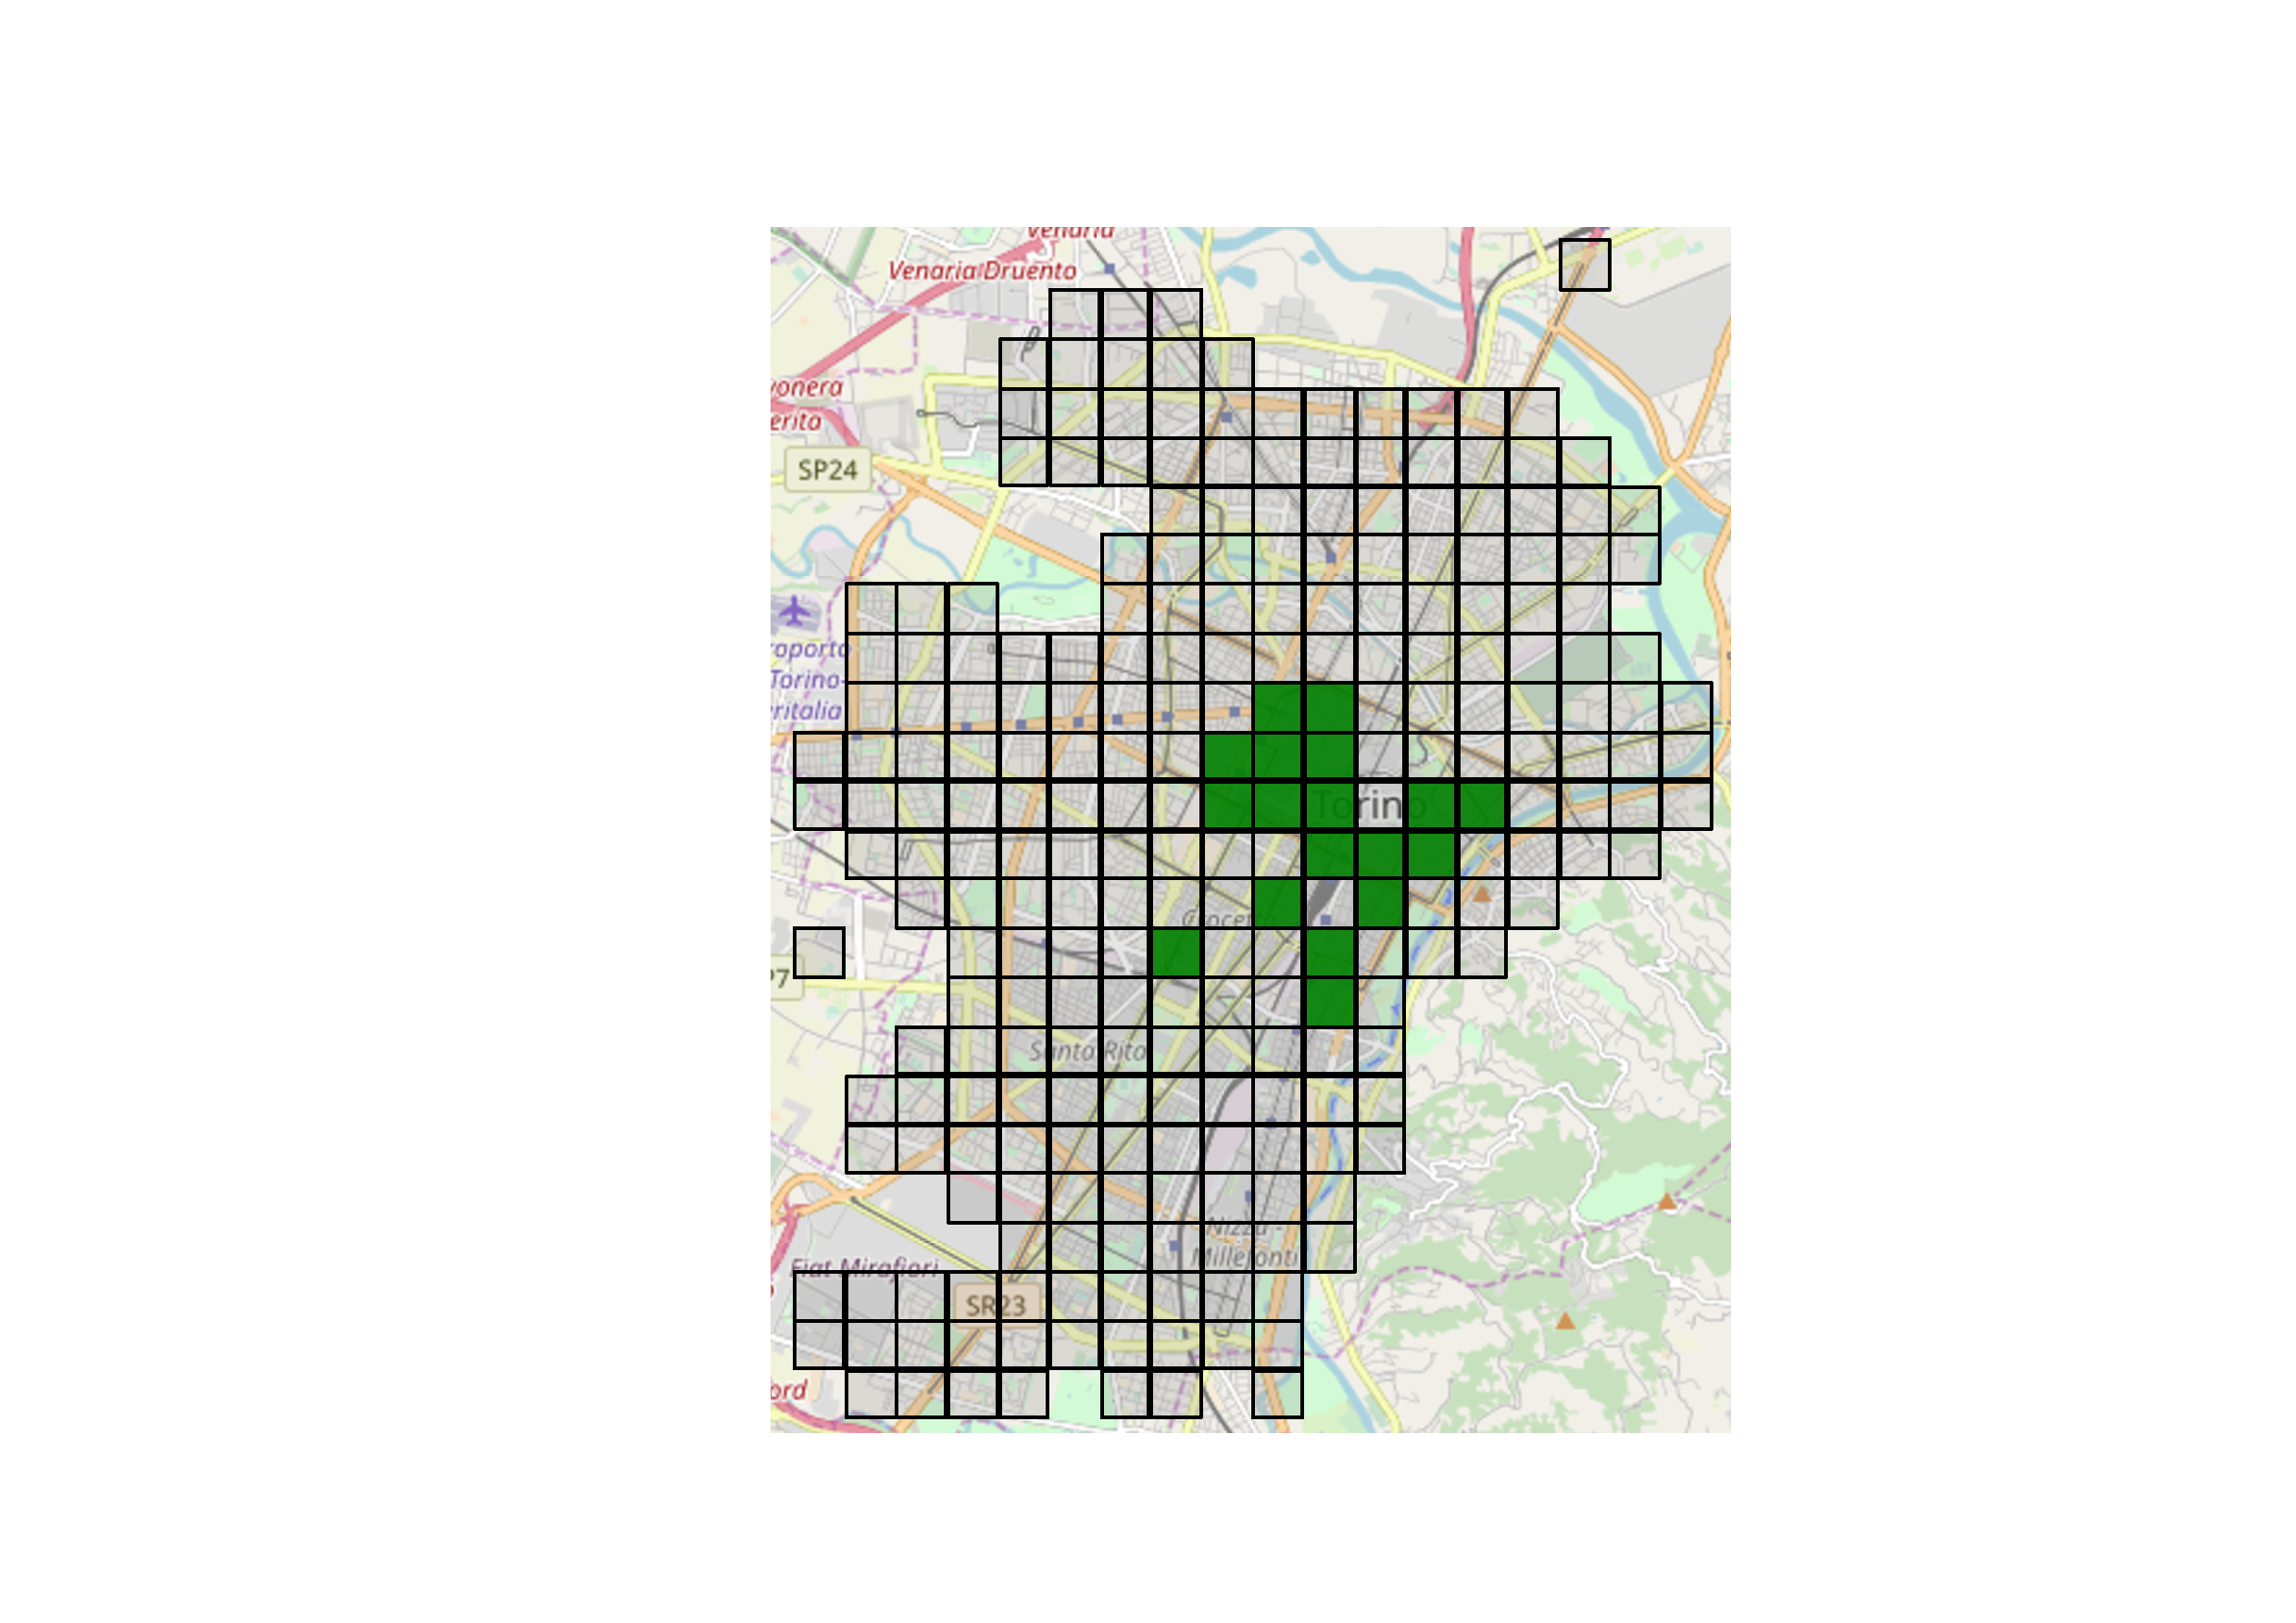
\includegraphics[width=0.3\columnwidth]{figures/NP_hybrid_18_Torino_placement.pdf}
        \label{fig:hm_max-parking_3}
    }
    \subfigure[\textit{Local Search}.]
    {
        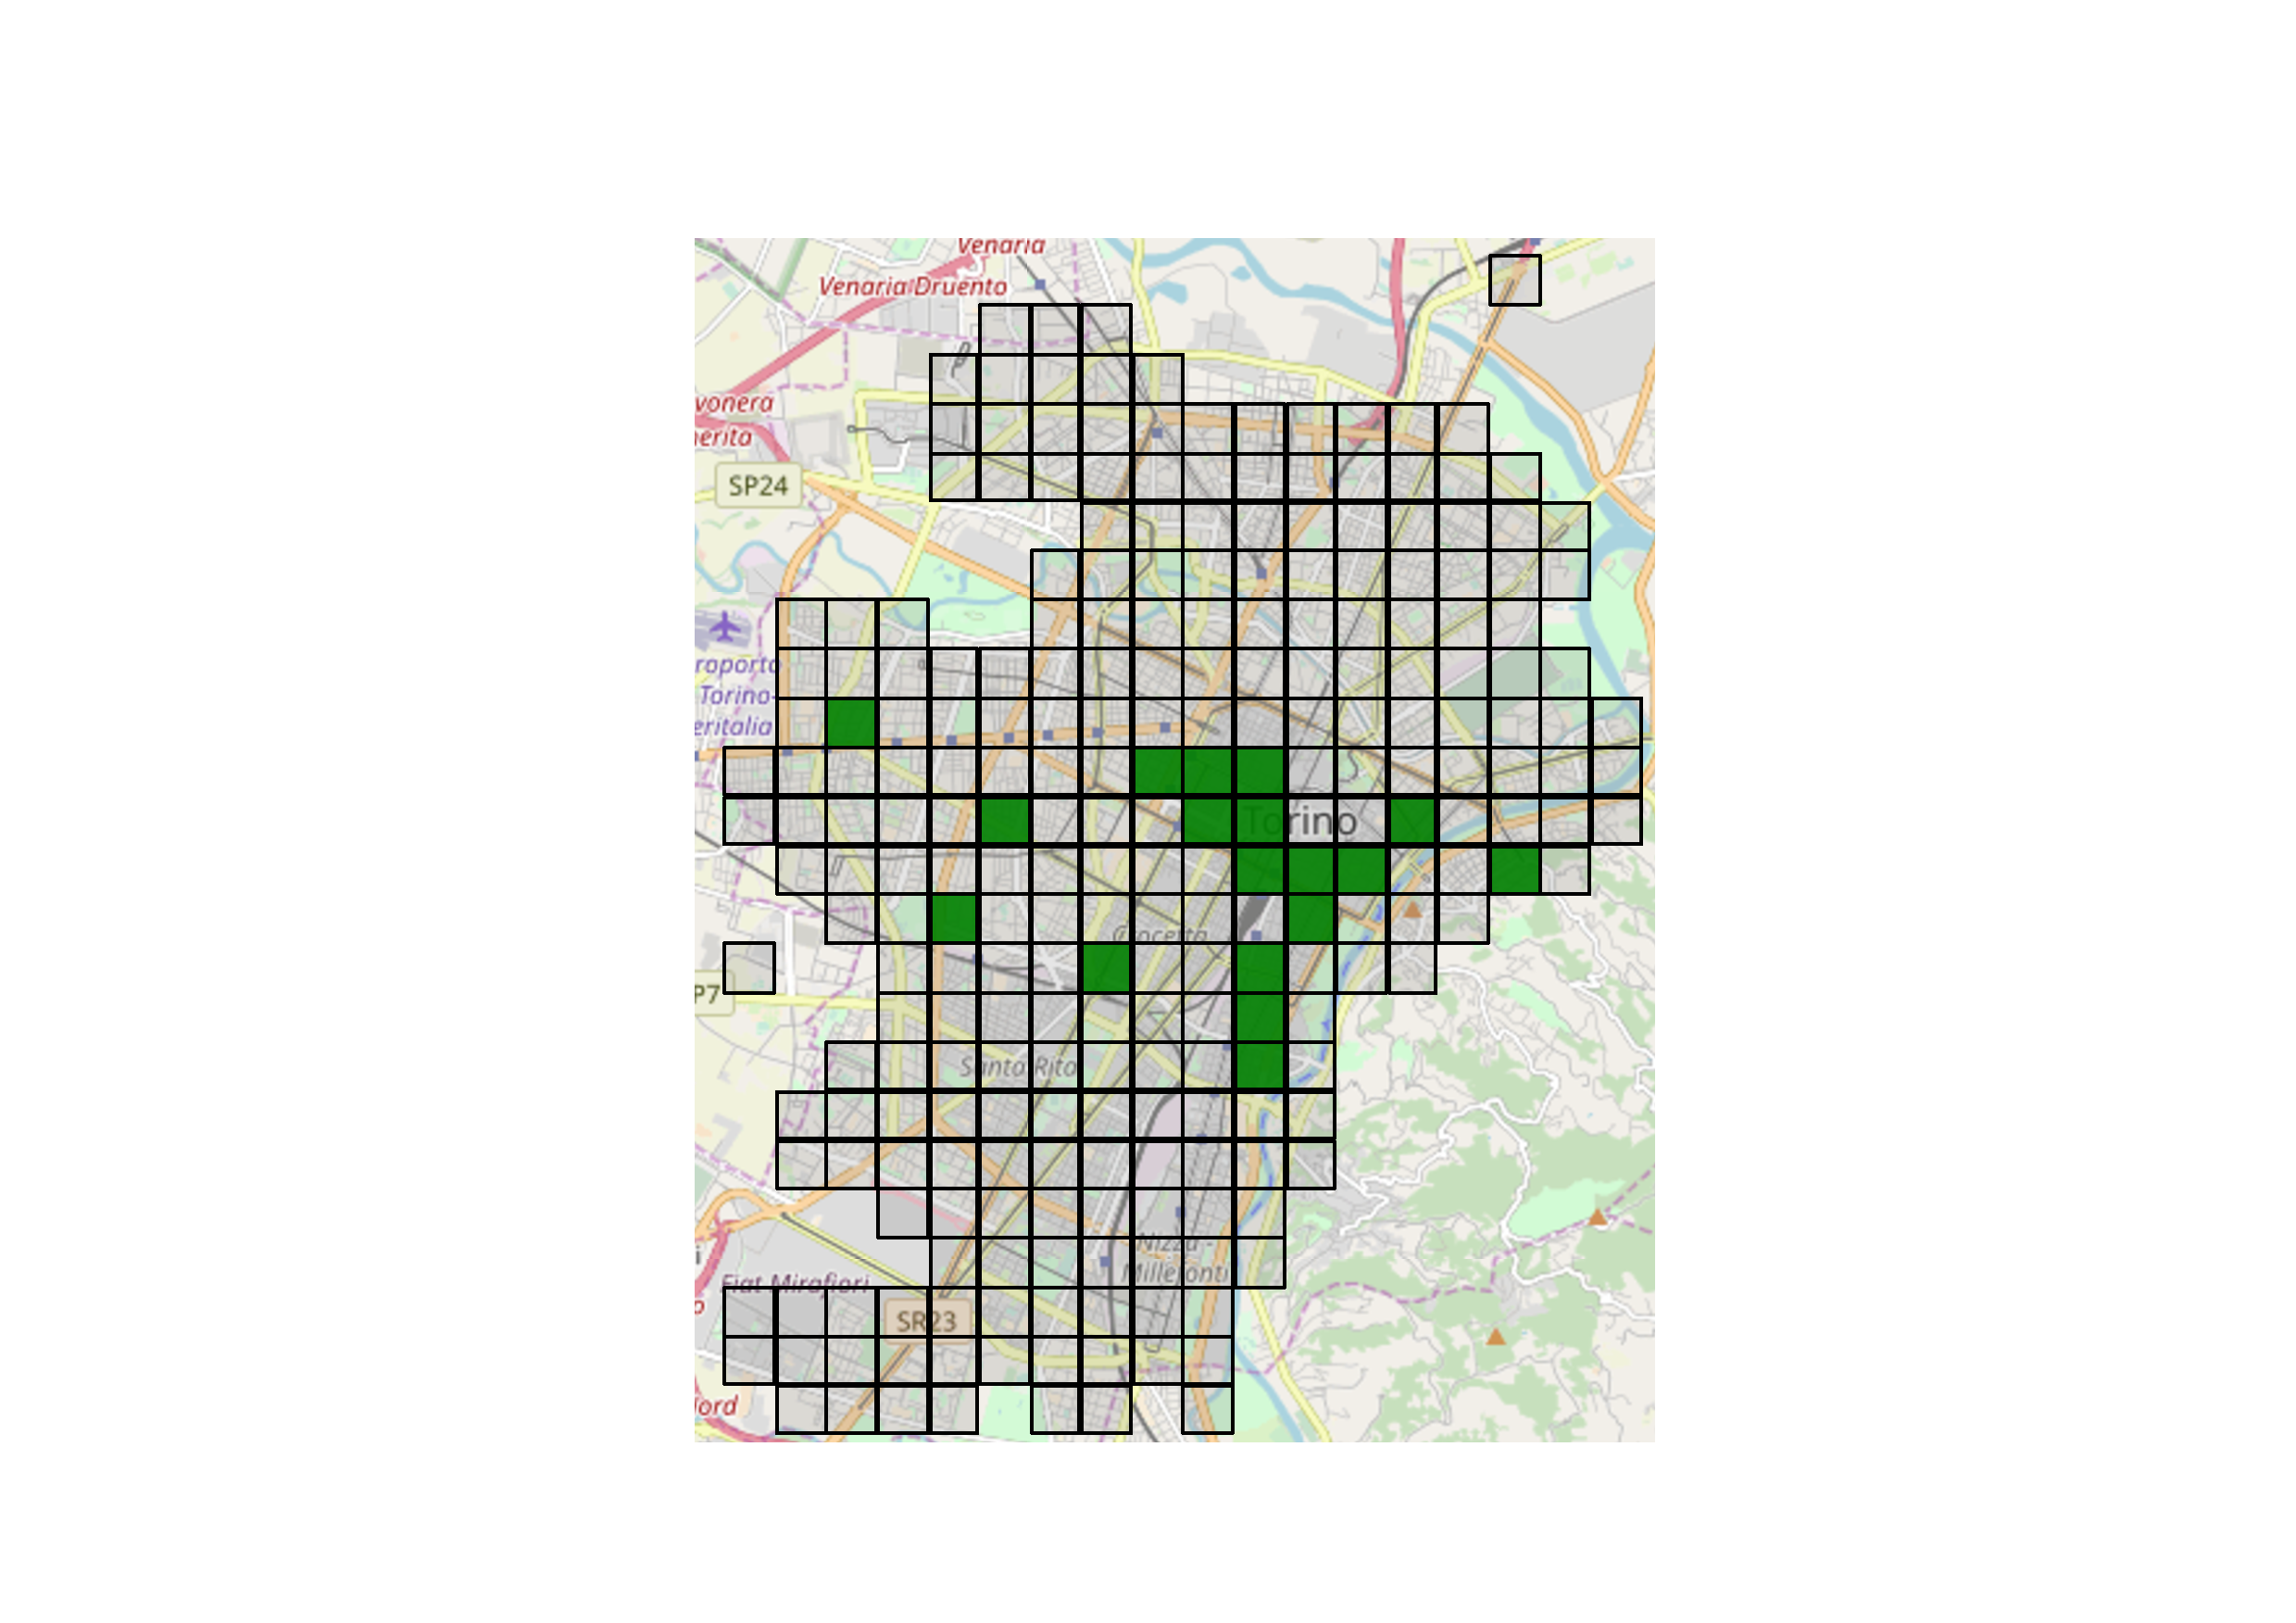
\includegraphics[width=0.3\columnwidth]{figures/LS_hybrid_18_Torino_placement.pdf}
        \label{fig:hm_local3}
    }
    \subfigure[\textit{Genetic} algorithm.]
    {
        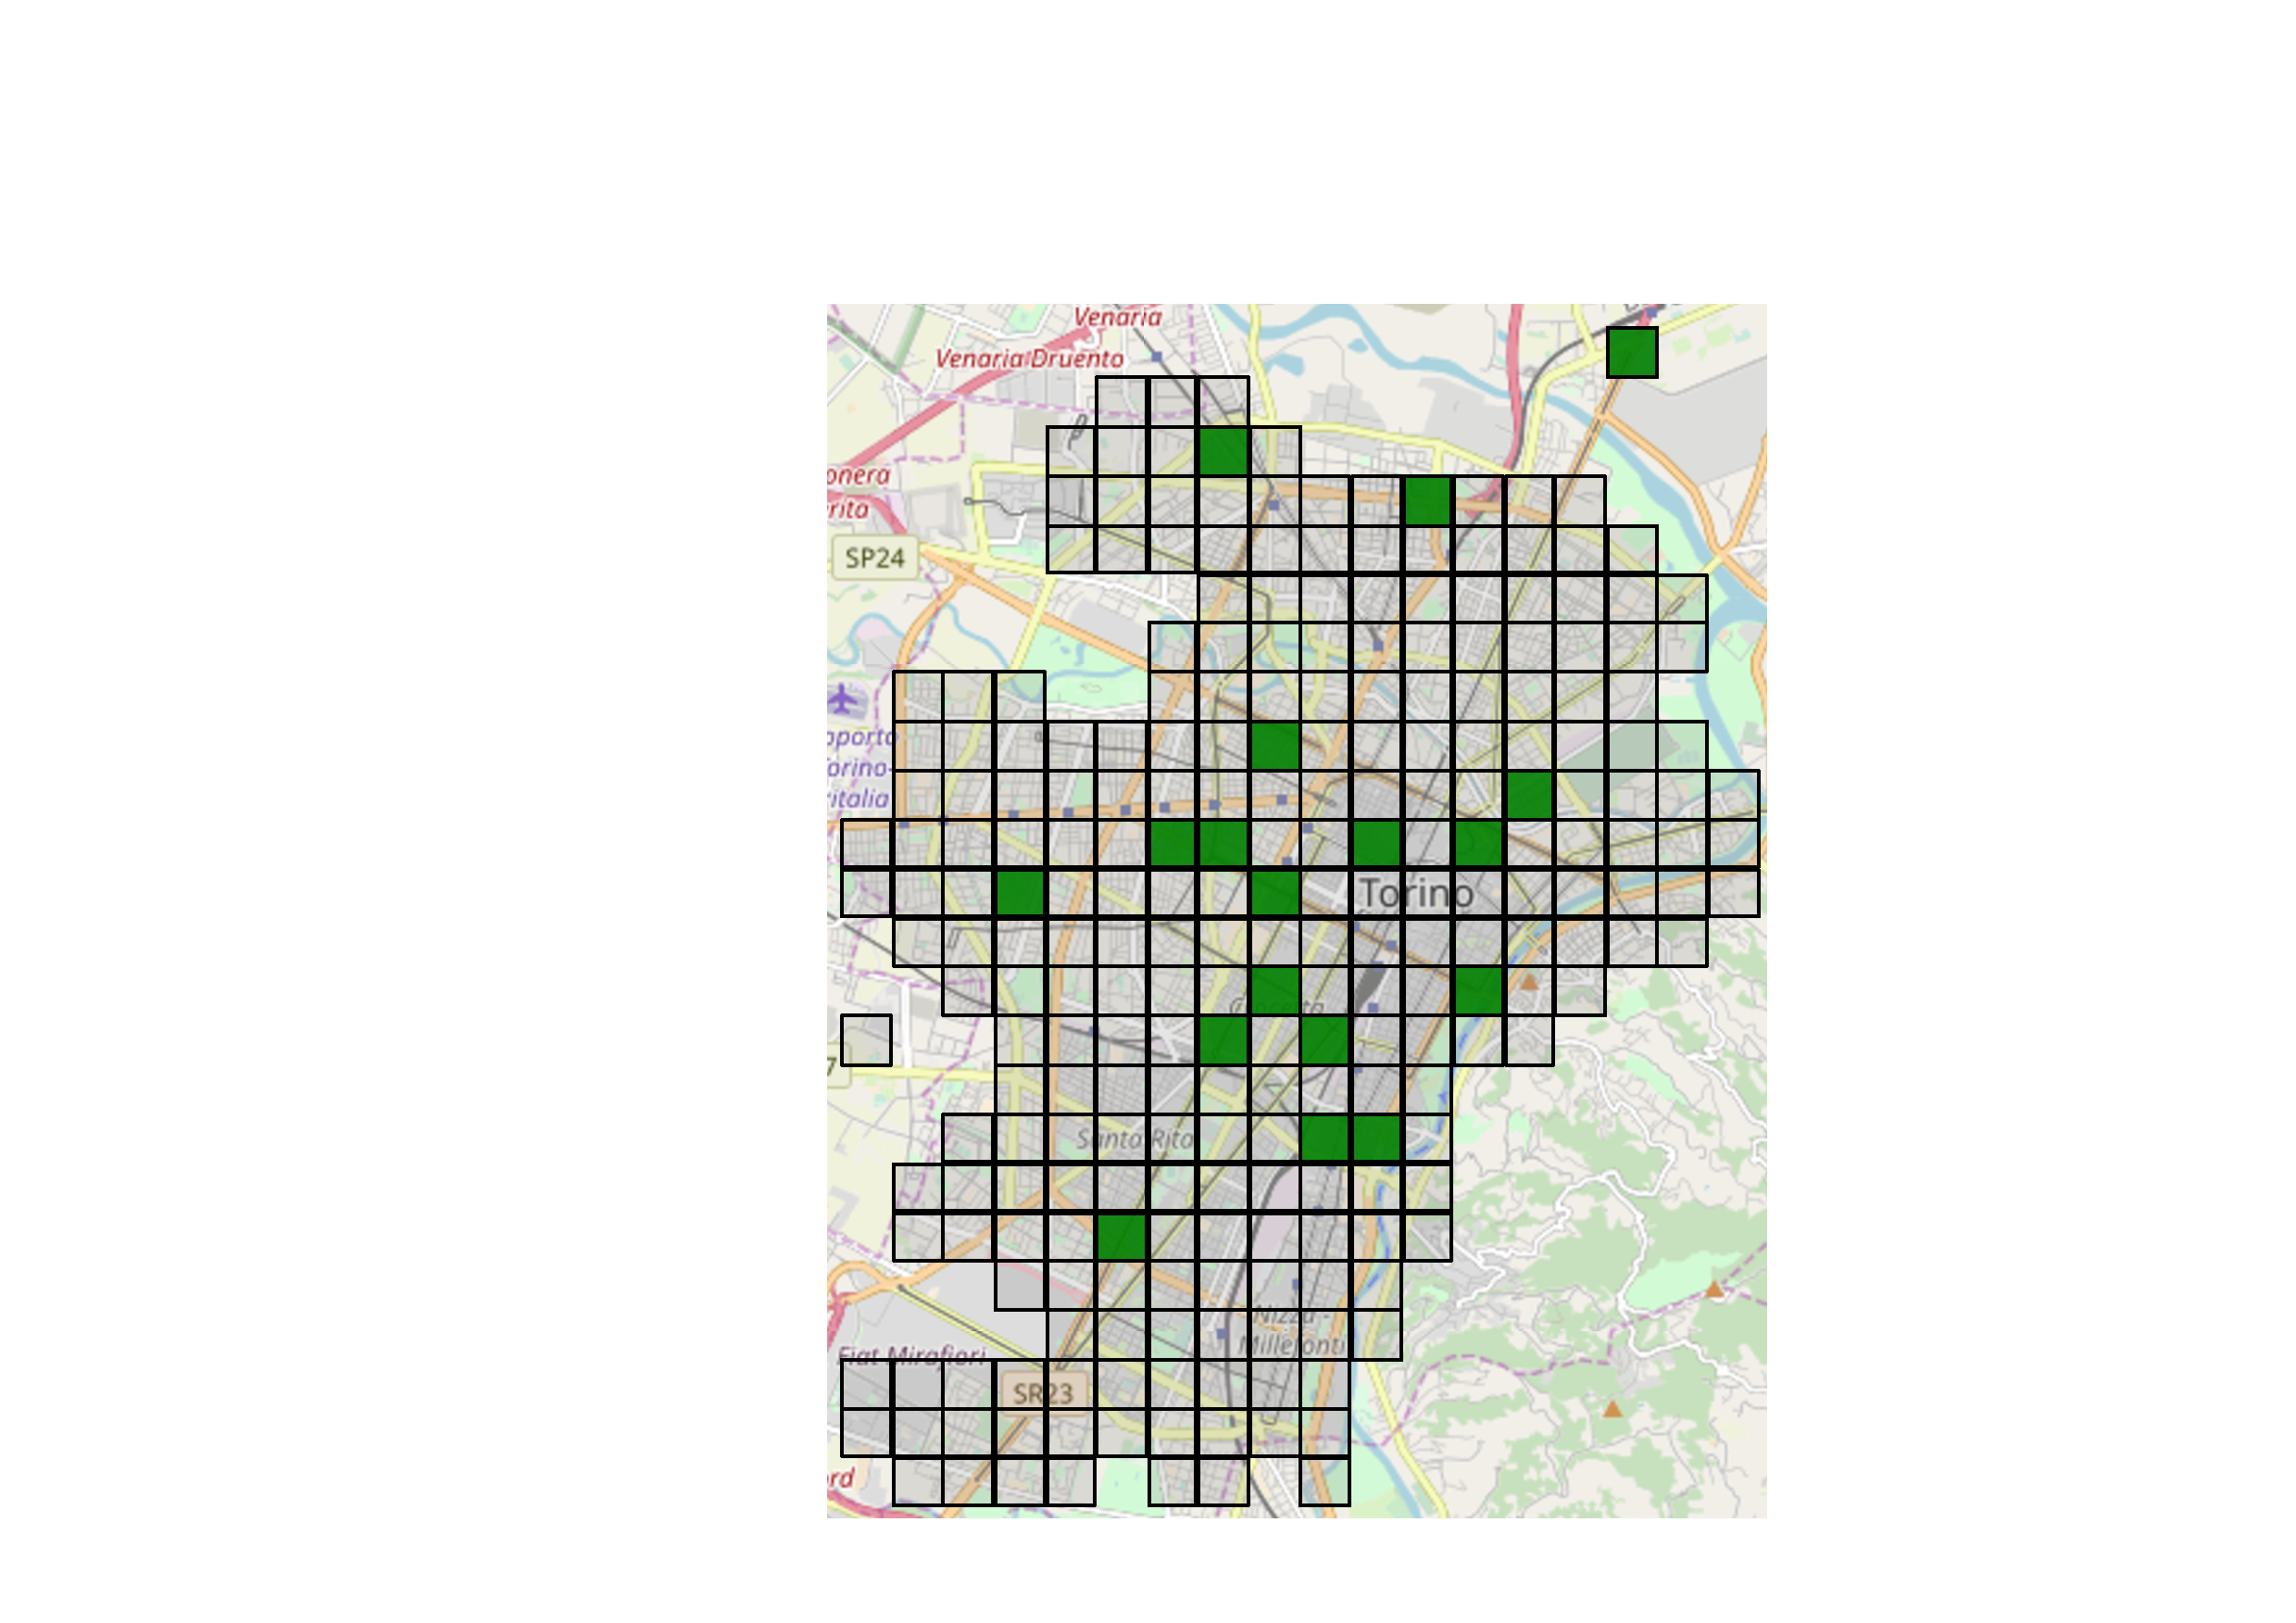
\includegraphics[width=0.3\columnwidth]{figures/GN_hybrid_18_Torino_placement.pdf}
        \label{fig:hm_genetico3}
    }
    \caption{Different placement of 18 zones (7\% of the total) for (a) Number of parkings per zone, (b) \textit{Local Search}  and (c) \textit{Genetic} solution. Darker areas have larger values.}
    \label{fig:maps}
\end{figure}

To give a feeling about the differences in the solutions found by different algorithms, Fig.~\ref{fig:maps} reports the solutions obtained with 7\% of the zones equipped with charging stations (i.e., $Z=18$ zones). %The upper right corner present in all figures refers to Turin airport (much further, in reality).  

\textit{Num parking} solution, Fig.~\ref{fig:hm_max-parking_3}, places most of the charging stations in downtown area and near the main train stations. 
\textit{Local Search}, Fig.~\ref{fig:hm_local3}, still has many zones in common with \textit{Num parking}, the solution it started from. It just spreads some charging station to cover also some remote zones.
The \textit{Genetic} algorithm, Fig.~\ref{fig:hm_genetico3}, shows very few zones in common with \textit{Num parking}. Charging stations are spread all over the city, still with more density in the city centre. %Moreover, the Turin airport is also a charging station zone, avoiding very long walks, a choice that the \textit{Local Search}, stuck in a local optimum, was not able to make. 



\subsection{Validation of optimised configurations}

\begin{figure}[t]
    \centering     %%% not \center
    \subfigure[Percentage of infeasible trips. Y-Axis is logarithmic.]
    {
        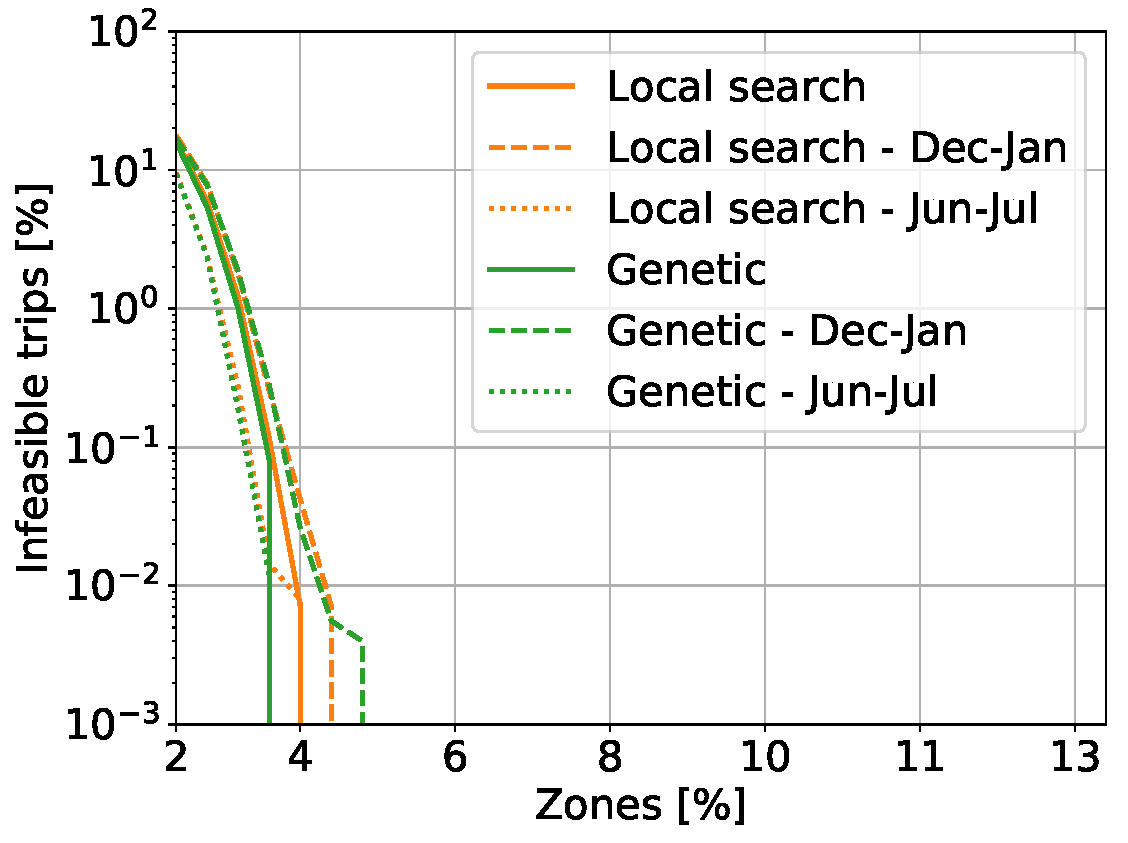
\includegraphics[width=0.45\columnwidth]{figures/Deaths_comparison.pdf}
        \label{fig:inf_validation}
    }
    \subfigure[Walked distance, averaged over all trips.]
    {
        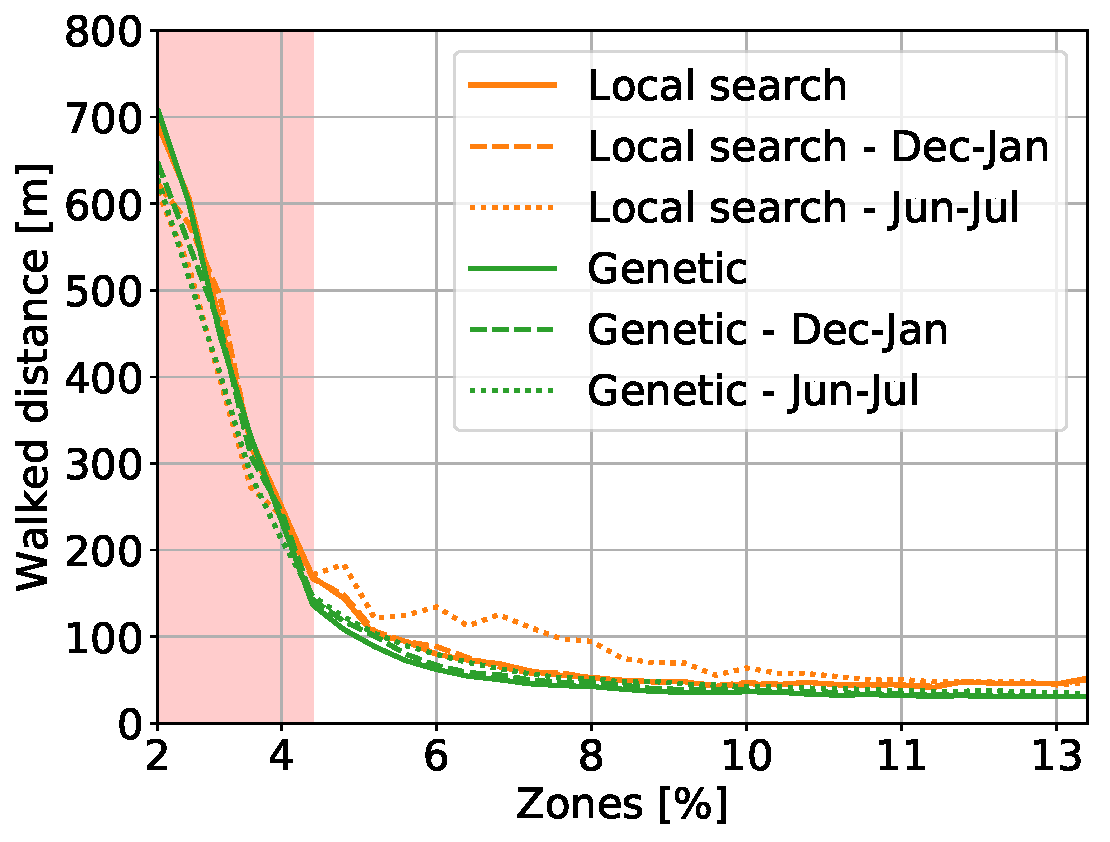
\includegraphics[width=0.45\columnwidth]{figures/TravelWithPenlaty_comparison.pdf}
        \label{fig:walked_validation}
    }

    \caption{Performance of the optimised configuration, tested on \DIFdelbeginFL \DIFdelFL{separate }\DIFdelendFL \DIFaddbeginFL \DIFaddFL{other }\DIFaddendFL 2 months long \DIFdelbeginFL \DIFdelFL{data}\DIFdelendFL \DIFaddbeginFL \DIFaddFL{data-sets}\DIFaddendFL .}
    \label{fig:validation}
\end{figure}

The optimised solutions presented in the previous section are built through data-driven simulations\DIFdelbegin \DIFdel{, hence may be over-fitting the data }\DIFdelend \DIFaddbegin \DIFadd{. Hence they might over-fit the data of the specific considered period }\DIFaddend and not be robust to \DIFdelbegin \DIFdel{in }\DIFdelend customers' habit changes. To validate our findings, we test \DIFdelbegin \DIFdel{our optimised placements by using a independent test trace}\DIFdelend \DIFaddbegin \DIFadd{the output placement configurations by using independent test traces}\DIFaddend , different from the one used to run the optimisation. 
\DIFdelbegin \DIFdel{For this, we use the two months of data of }\DIFdelend %DIF >  For this, we use the two different periods of two months: the latter selected in December 2017 and January 2018, collected in Turin again. For these two months we record 128\,780 rentals (3\% more trips than before). Instead the former takes in account June 2017 and July 2018 considering 101\,049 actual rentals. In this period the number of bookings 8\% lower due to beginning of European Summer. Those periods present different customers' habits, a hard challenge for the optimised configurations.
\DIFaddbegin \DIFadd{We rely on two traces collected in Turin in two different periods of the year: one in summer, from June to July 2017; the other in winter, from }\DIFaddend December 2017 \DIFdelbegin \DIFdel{and January 2018, collected in Turin again. For these two months we record 128\,780 rentals (3\% more trips than before).This period includes many holidays, when customers ' habits are different, a hard }\DIFdelend \DIFaddbegin \DIFadd{to January 2018. We focus on these two periods since in summer and near Christmas holidays the users may exhibit different habits (e.g., customers may rent the cars to go to parks and swimming pools during summer). These anomalies may represent a }\DIFaddend challenge for the optimised configurations.
\DIFaddbegin \DIFadd{In the summer trace we record about  100\,000 rentals, while in the winter one 128\,000 rentals (respectively 8\% less and 3\% more with respect to the September/October trace). }\DIFaddend We compute the \DIFdelbegin \DIFdel{charging optimal station placement }\DIFdelend \DIFaddbegin \DIFadd{best station placement considering the September and October 2017 trace, and test system performance }\DIFaddend using the \DIFdelbegin \DIFdel{first two months of trips, and then we test again its performance on the second two months of trips}\DIFdelend \DIFaddbegin \DIFadd{summer and winter traces}\DIFaddend .  

Fig.~\ref{fig:validation} \DIFdelbegin \DIFdel{reports resultsfor the optimised trace (same curves as in Fig.~\ref{fig:optimized_metrics}), and the new test trace. Both }\DIFdelend \DIFaddbegin \DIFadd{compares results. We consider both }\DIFaddend \textit{Local Search} and \textit{Genetic} \DIFdelbegin \DIFdel{are considered and tested}\DIFdelend \DIFaddbegin \DIFadd{algorithms}\DIFaddend .
%\lv{diciamo negligibili come walked distance. Come infeasible trips cambiano, piu delle figure mostrate sopra sugli infeasible trips. Ma trattandosi di poche morti, anche solo la parte randomica va a influire abbastanza}
%As we can see, both figures have curves whit similar trends
\DIFdelbegin \DIFdel{Differences }\DIFdelend %DIF >  Differences are negligible, showing that optimisation results are robust. For example, for 13\% of zones and considering \textit{Genetic} algorithm, the walked distance on the test is just 2\,m above the one in the optimised trace. 
\DIFaddbegin \DIFadd{In almost all cases, differences }\DIFaddend are negligible, showing that \DIFdelbegin \DIFdel{optimisation results are }\DIFdelend \DIFaddbegin \DIFadd{the solution is }\DIFaddend robust. For example, for 13\% of zones and considering \textit{Genetic} algorithm, the walked distance on the \DIFdelbegin \DIFdel{test is }\DIFdelend \DIFaddbegin \DIFadd{tests are }\DIFaddend just 2\,m above \DIFdelbegin \DIFdel{the one in the optimised trace . 
}\DIFdelend \DIFaddbegin \DIFadd{those in the trace used for optimisation. Notice how in June and July the }\textit{\DIFadd{Local Search}} \DIFadd{behaves worse than other cases: this is possibly due to the different mobility patterns in summer, while the Local Search solution could still be too related to the number of parkings in September-October. On the other hand, the solution found by the global genetic algorithm is robust.
%DIF > In any case this behaviour is noticeable considering few charging stations: considering more than 13\% of zones the placements have the same performances.
}

\DIFaddend %In the test set, the number of infeasible trips goes to 0 needing up to 3 additional zones for both genetic and local search. Regarding the walked distance, for 13\% of zones, the genetic algorithm walked distance on the test is just 2\,m above the one optimized on the original dataset. 
%Concluding, our placement solutions do not overfit the trace used for the designing and seem robust with respect to the change of habits.

\DIFaddbegin \section{\DIFadd{Discussion and Implication}}
\label{sec:discussion}

\DIFadd{The mobility model we use for optimising the placement of charging station reflects customers habits. However, there are other aspects of car sharing system design that one could consider. In the following, we briefly discuss two of them.
}

\subsection{\textbf{\DIFadd{Scalability}}}

\DIFadd{We built the events trace from real rentals in the analysed city. By using this data we use simulations to study placement solutions which cope with the current amount of traffic and usage of the FFCS. While in a short term this solution is optimal, we have no guarantee whether it will be valid in the future in case of a strong increase in the car sharing usage, e.g., when popularity increases by orders of magnitude. To tackle this problem, we can still leverage rental data to infer a model about car sharing usage patterns in time and space, where the demand can be easily controlled by increasing the frequency of rentals. This model can then be used to create synthetic traces with an increasing car sharing demand, and use simulations to assess overall system performance. As such, the methodology we designed is generic and could be used to study different }\textit{\DIFadd{What-If}} \DIFadd{cases.
}

\DIFadd{Directly linked to the scalability problem, another important aspect is the possibility to add new charging stations when car sharing demand changes. 
By analysing the data collected by UMAP, our methodology can be used to consider the greedy placement of new charging stations on the top of those already present.
}

\subsection{\textbf{\DIFadd{Economical Aspects}}}


\DIFadd{Economical aspects play too a key role in the placement decision process. In this work, we decided to study only the feasibility of the EV based FFCS system design by considering as few charging stations as possible, leaving for a next step the detailed cost estimation. The cost of the infrastructure creation and management can largely vary depending on different variables such as country, city, incentives. 
Related to this first class of costs, authors in~\mbox{%DIFAUXCMD
\cite{USAInstallCost} }%DIFAUXCMD
give a first estimation of installation cost, which can be of up to 5\,500~USD per pole in the USA. 
While analysing these costs and developing a business plan, it is also important to evaluate which parties could be interested on running a business around it, e.g., either the municipality or a third party company could offer the infrastructure as a service to FFCS providers and other customers with electric vehicles.  
}

\DIFadd{The second group of variables consider the earnings models and the variable costs of the FFCS provider, like energy and cars. This kind of data requires a careful analysis to get a reliable estimation. Authors in~\mbox{%DIFAUXCMD
\cite{8_Wagner2015DataAF} }%DIFAUXCMD
suppose a marginal profit of 75\% of the fare considering a FFCS provider in the city of Vancouver. However, to correctly estimate the net profit several aspects need to be considered, such as the fee per minute, the actual duration of the rental costs and incentives for reroutes.
}

\DIFadd{Given that, we are currently working on a more complete model to better study the economical impact of electrification by including in the simulator a precise cost model. 
}


\DIFaddend \section{Conclusions}
\label{sec:conclusion}

Designing an electric free floating car sharing systems leads to many interesting problems and trade-off between usability, costs and benefits for the customers. 
In this work, we built on actual rental traces to study via accurate simulations the impact of different charging stations placement and charging policies. 
We considered Turin as a case study, using 2 months of rentals recorded from a currently operational FFCS that we use to run trace driven simulations.

%More in details we defined a meta-heuristic algorithm placing the charging stations. Then we minimised the system leaks and users discomfort through an hill climb local search algorithm, after we compared those result with the optimisation coming from a genetic algorithm and finally we validated our output placement with a different trace.

We have shown that few charging stations are enough to make the system self-sustainable. Important is the customers collaborations, so that they voluntarily returns to the cars to charging stations when available
\DIFdelbegin \DIFdel{.
}%DIFDELCMD < 

%DIFDELCMD < %%%
\DIFdelend Our data driven results show that just $5\%$ of the city zones that are equipped with charging stations (13 in total, 52 poles) make all trips feasible with an electric car fleet. Moreover, through a charging station placement based on a genetic optimisation algorithm, it is possible to minimise the discomfort for the customers that would be (rarely) asked to bring the car for charging. For example, with 18 charging stations (72 poles in total), on average a customer would walk only 40\,m to reach its desired destination. 
%DIF < lv{18 e' lo stesso numero che abbiamo usato sopra per la visualizzazione}
\DIFaddbegin \DIFadd{While these numbers will change in different cities, the data driven approach we propose naturally fits the global optimisation algorithm that is able to optimise placement while considering complex customers habits.
}\DIFaddend 



%These results are obtained also thanks to the users collaboration by returning the car to a nearby charging station, and whenever the battery level drops below a target threshold.

%the performances of the meta-heuristic placement are improved by the optimisation algorithms. 
%The system can auto-sustain itself with a smaller number of charging stations, 3.8\% with a local search and 3.5\% of zones with genetic algorithm (respectively 9 and 10 zones).
%Both algorithm tried to move the charging stations from downtown to high population density areas.
%Finally we have validated our results using a different trace with a different users' patterns (in the same city with the same fleet size) pointing out how the algorithms was not overfitted: the stability condition was reached by adding 3 zones, while the difference of walked distance is 2 m only. 

%For instance our results show how the intuition coming out the data observation might be still improved using basic optimisation algorithms leading to conditions in which systems sustainability and users' discomfort are improved. 

We leave for future work the simulations of scenarios with new technologies, such as deployment of faster charging poles and larger batteries, and the scalability in terms of number of customers and fleet size.
We believe that our approach, based on data and accurate simulations is very promising to design and understand electric FFCS systems in future smart cities\DIFaddbegin \DIFadd{, provided actual data is available}\DIFaddend .


\bibliographystyle{elsarticle-num}
\doublespacing
\bibliography{paper}


\appendix
%This is an appendix
\section{Placement optimisation for \textit{Needed} return policy}
\label{sec:needed}

 
 \begin{figure}[h]
     \centering     %%% not \center
    \subfigure[Percentage of infeasible trips. Y-Axis is logarithmic.]
    {
        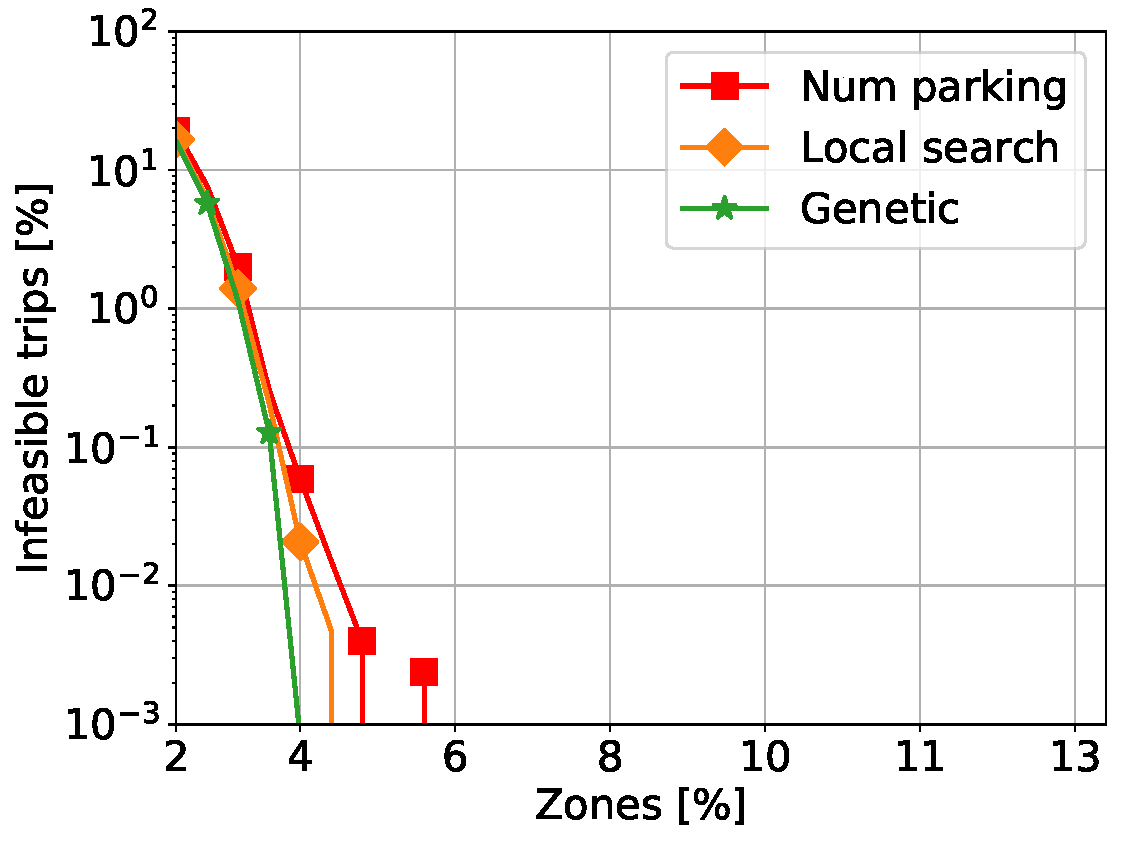
\includegraphics[width=0.45\textwidth]{figures/Needed_Deaths.pdf}
        \label{fig:optimized_deaths_Needed}
    }     
     \subfigure[Walked distance, averaged over all trips.]
     {
         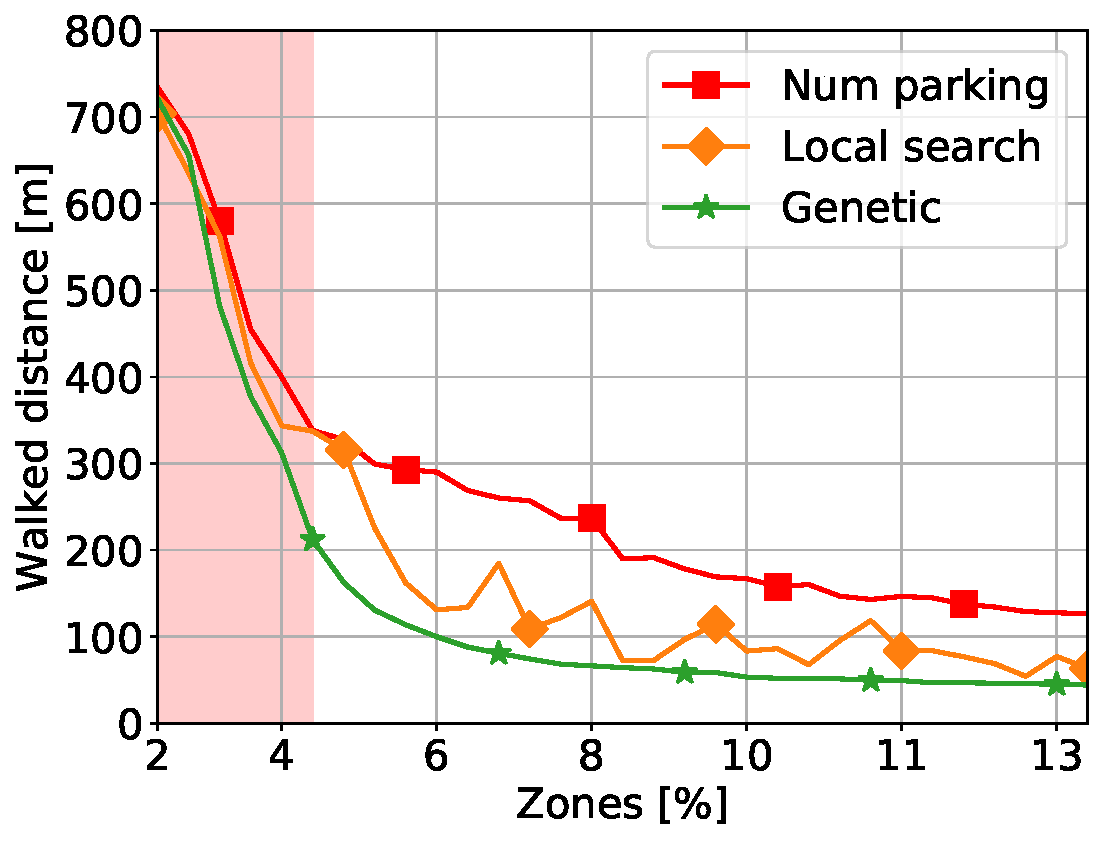
\includegraphics[width=0.45\textwidth]{figures/Needed_TravelWithPenlaty.pdf}
         \label{fig:wwd_Needed}
     }
     \caption{Objective metrics to minimise in the optimisation - with \textit{Needed} return policy}
    \label{fig:optimized_metrics_needed}
 \end{figure}

Here  we briefly report the results for the optimisation experiments of the \textit{Needed} policy.
We followed the same procedure explained in Sec.~\ref{sec:opt} for the \textit{Hybrid} return policy. As in that case, the genetic algorithm is able to largely optimise the solution, as reported in Fig.~\ref{fig:optimized_metrics_needed}, with \textit{local searches} stuck in local minima. 
In particular, for the walked distance (Fig.~\ref{fig:wwd_Needed}), the genetic algorithm is able lower it from 136\,m to 45\,m at 13\% of zones. Still, it doesn't reach the performance of the \textit{Hybrid} policy, i.e., 30\,m at 13\% of zones.


%Fig.~\ref{fig:optimized_deaths_Needed}, the infeasible trips perform better with the \textit{Genetic} and the \textit{Local search} getting to zero infeasible trips with \dg{4.3}\% and \dg{7.7}  respectively.
%Looking at the walked distance in Fig.~\ref{fig:wwd_Needed}, we can see that both optimizers perform much better with respect to the \textit{Num Parking} getting lower than 100 m. 

  \begin{figure}[t]
     \subfigure[Charges percentage.]
     {
         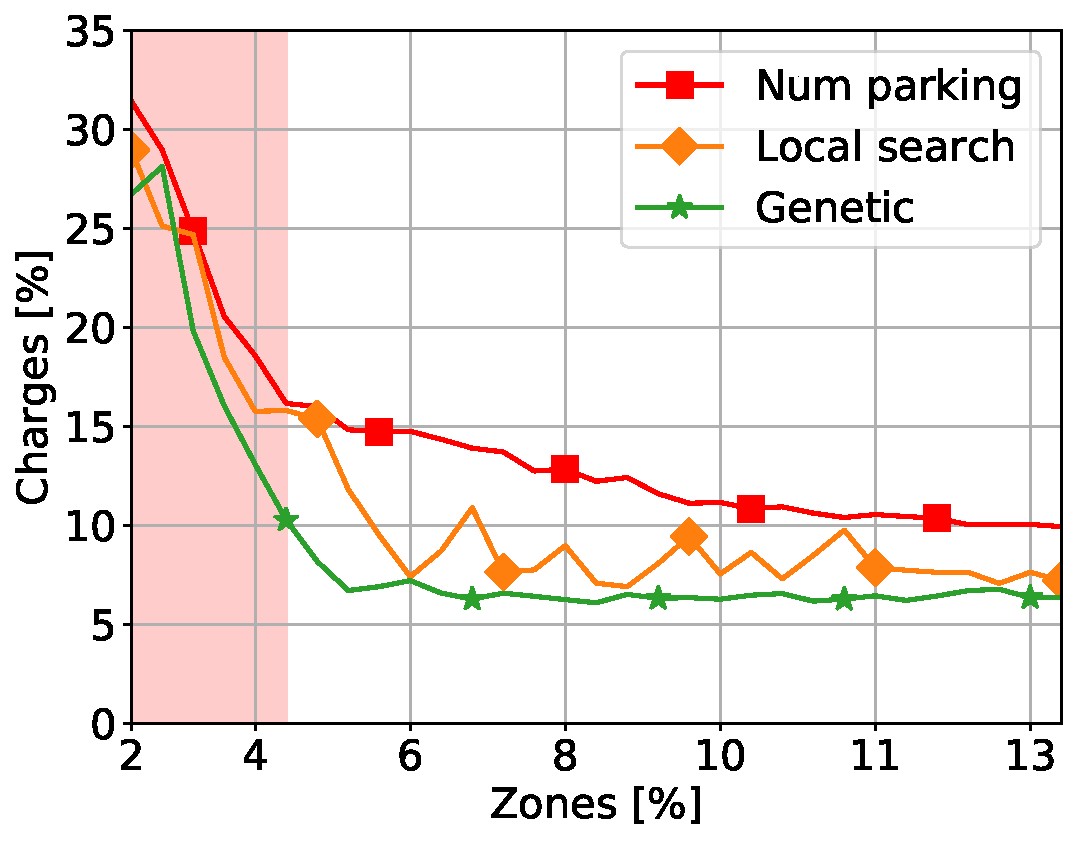
\includegraphics[width=0.45\textwidth]{figures/Needed_AmountRechargePerc.pdf}
         \label{fig:recharge_Needed}
     }
    \subfigure[Average state of charge.]
    {         
        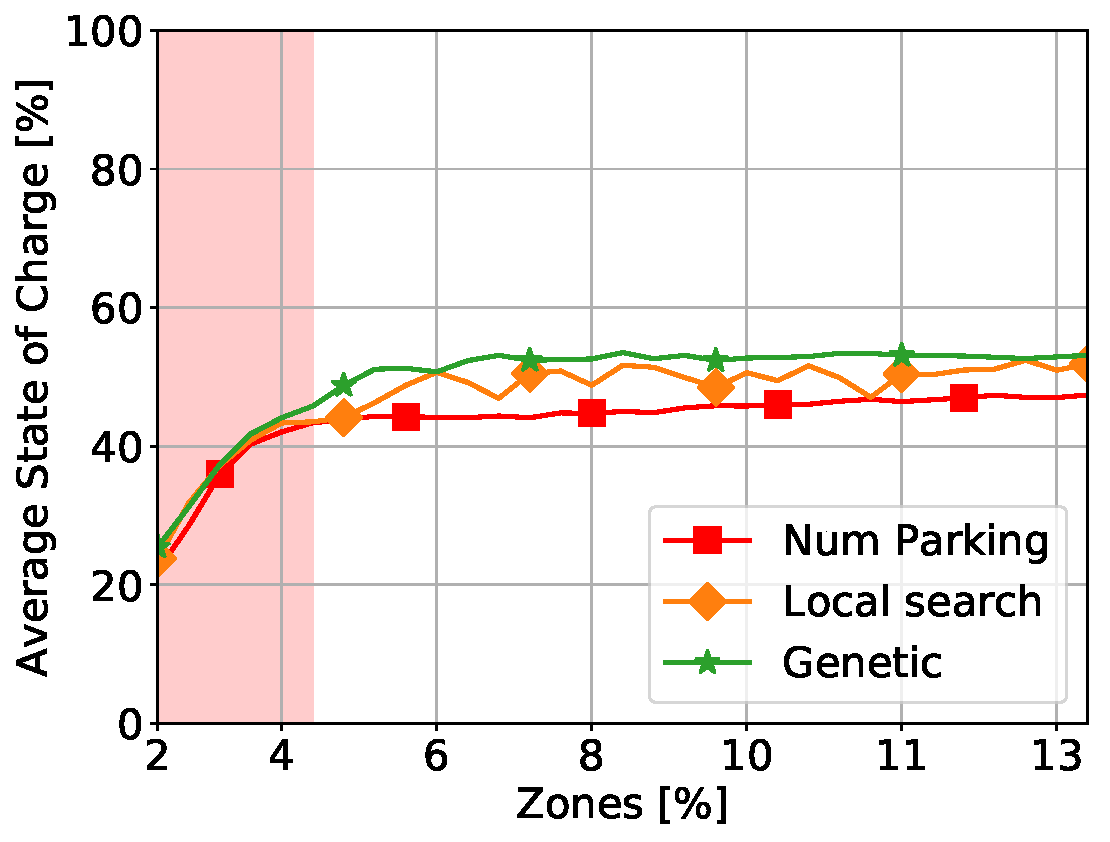
\includegraphics[width=0.45\textwidth]{figures/AvgSOC_comparison_N}
        \label{fig:asoc_Needed}
    }     
     \subfigure[Rerouted trips percentage.]
     {
         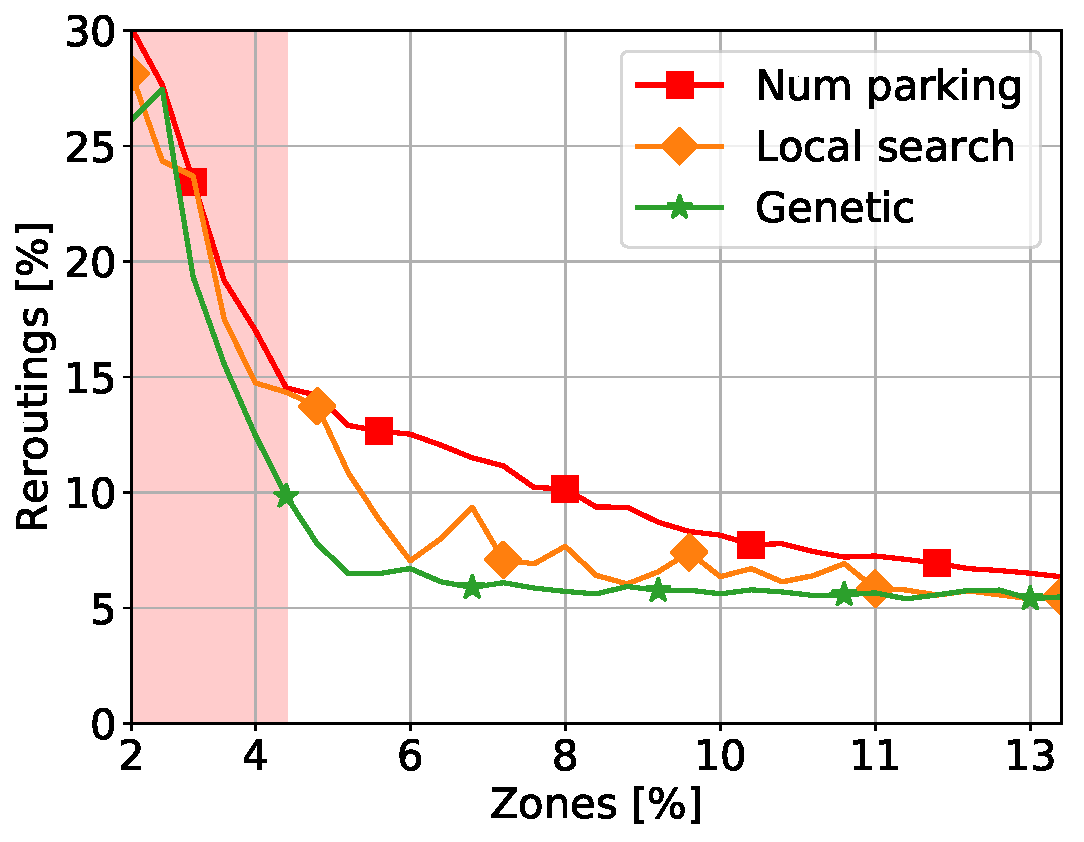
\includegraphics[width=0.45\textwidth]{figures/Needed_ReroutePerc.pdf}
         \label{fig:reroute_Needed}
     }
     \quad
     \subfigure[Walked distance when rerouted.]
     {
         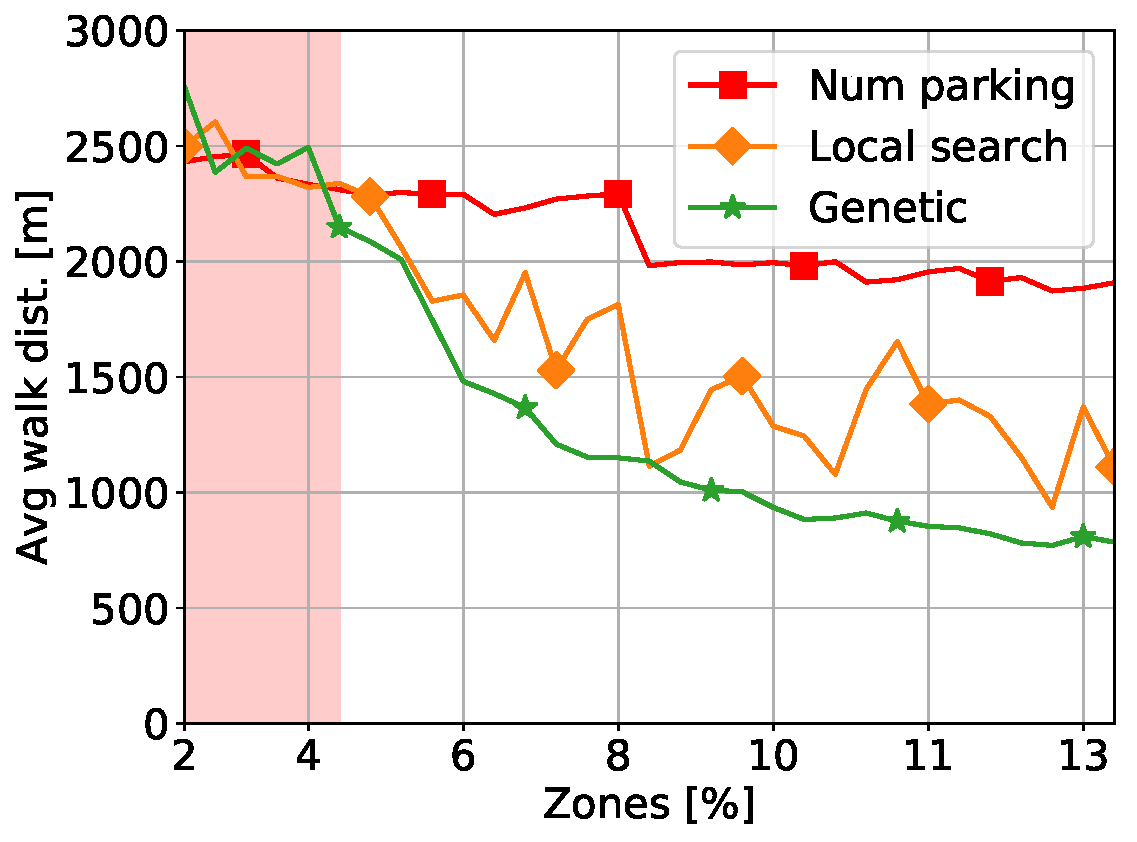
\includegraphics[width=0.47\textwidth]{figures/Needed_AvgWalkedDistance.pdf}
         \label{fig:awd_Needed}
     }
     \caption{\textit{Genetic} and \textit{local search} optimization results for metrics of interests (\textit{Needed} return policy adopted).}
     \label{fig:opt_needed}

\end{figure}

Fig~\ref{fig:opt_needed} reports the other user discomfort metrics.
The two optimisation algorithms reduce the charge events (Fig~\ref{fig:recharge_Needed}).
%The \textit{Genetic} algorithm shows the best performance with a probability the lowest probability of 6\% when 13\% of the zones are equipped with charging stations. 
%Since the car are recharged less frequently with respect to the \textit{Hybrid} policy it is interesting to evaluate the impact on the \textit{Average Stage of Charge}. Fig.~\ref{fig:asoc_Needed} reports this metric for the different placement algorithms.  As we expected, the \textit{Average Stage of Charge} is lower with respect to the \textit{Hybrid policy}. Interestingly, for both optimized solutions this value saturate almost immediately at \dg{55}\% in the feasible region. Moreover, despite in Fig.~\ref{fig:recharge_Needed} we saw that in the optimized solutions we recharge less frequent the car, 
However,  the average state of charge (Fig.~\ref{fig:asoc_Needed}) is always higher in the optimised solutions than in the \textit{Num parking} configuration. This further demonstrates that a smarter placement allows the car to get more energy for each charge.
%with an opposite trend with respect to Fig~\ref{fig:recharge_Hybrid},
%Finally, we evaluate the users discomfort metrics in terms of rerouting probability and the average distance an user has to walk when rerouted.
Fig.~\ref{fig:reroute_Needed} reports the rerouting percentage for the different algorithms. As expected, the values are larger than with the \textit{Hybrid} policy, since no opportunistic charge is performed. 
%This different is particularly evident when a few charging stations are present e.g., with 5\% of charging stations the rerouting are \dg{14}\% for the \textit{Num parking} heuristic, \dg{14}\% for the \textit{Local search}, and \dg{6}\% for the \textit{Genetic} algorithm. 
However, the genetic algorithm is able to quickly reach a small value of reroutings, hence better exploiting every charge possibility. 
%without showing further improvements while increasing the percentage of charging stations applied. 
Finally, we analyse the distance a user has to walk when rerouted (Fig.~\ref{fig:awd_Needed}). Here, with respect to the \textit{Hybrid} policy case, the \textit{local search} shows larger deviations from the \textit{Num parking}. The genetic algorithm reaches values of about 800\,m, even below the ones reached with the \textit{Hybrid} policy.

In conclusion, within this range of zones equipped with charging stations, a smart placement with the \textit{Needed} policy approaches the \textit{Hybrid} policy results.  
%Therefore, anche se gli utenti non sono tutti collaborativi, il sistema va bene lo stesso se ottimizzato.



 
 
 
 




\end{document}
